\RequirePackage{snapshot}
\documentclass[a4paper, 11pt, tipotesi=topfront]{toptesi}

\usepackage[latin1]{inputenc}
\usepackage[italian]{babel}

\usepackage{amssymb}
\usepackage{subfigure}
\usepackage{topfront}
\usepackage{upgreek}

\usepackage{algorithm}

\usepackage{algpseudocode}


%Opzioni
\floatname{algorithm}{Algoritmo}
\renewcommand{\algorithmicrequire}{\textbf{Input:}}
\renewcommand{\algorithmicensure}{\textbf{Input:}}

\includeonly{
	sommario, 	%
	capitolo1,	%
	capitolo2,	%
	capitolo3,	%
	capitolo4,
	conclusioni,	%
	appendici, 	%
	bibliografia	%
 }

\begin{document}

% Questo � un commento

\begin{frontespizio}
\facolta[III]{Ingegneria}
\corsodilaurea{Ingegneria Informatica}
\NomeMonografia{Monografia di tirocinio}
\monografia{Texture mapping}
\sottotitolo{Texture mapping applicato al calcolo dell'ambient occlusion}
\candidato{Fabrizio Destro}
\sedutadilaurea{Ottobre 2011}
\logosede{./images/polito}
\end{frontespizio}

\tableofcontents

\chapter*{Sommario}
\addcontentsline{toc}{chapter}{Sommario}	%In questo modo compare nell'indice ma senza numerazione
Lo scopo di questa monografia � di esporre in maniera chiara e concisa l'attivit� svolta all'interno dell'azienda Seac02.  Per aiutare il lettore nella consultazione, la monografia � stata suddivisa in tre parti principali la prima che descrive l'azienda e le attivit� svolte, la seconda in cui si parla dell'analisi e della fase progettuale e la terza in cui si affrontano i dettagli di realizzazione dell'applicativo. Un'ultima parte � dedicata al commento sul lavoro svolto e uno sguardo critico al risultato ottenuto, con un occhio ai possibili sviluppi futuri.

L'argomento su cui verte la monografia � la realizzazione di un applicativo per il calcolo dell'ambient occlusion e la creazione della texture associata. L'ambient occlusion � un metodo di ombreggiatura utilizzato nella grafica computerizzata per conferire realismo ai modelli di riflessione locale. La texture � un'immagine bidimensionale utilizzata per rivestire la superficie di un oggetto virtuale, � utilizzata per aggiungere dettagli al modello. Nel nostro caso la texture � utilizzata per rappresentare l'ombreggiatura locale del modello.

Questo applicativo dovr� agire su un gran numero di modelli in maniera automatica, senza nessun tipo d'intervento umano. Dovr� quindi essere in grado di determinare una parametrizzazione valida per il modello, di campionare l'occlusione sull'intera superficie virtuale e scrivere il risultato su una texture.

L'obiettivo � quello di risolvere alcune problematiche presenti nel lavoro fin qui svolto. Queste riguardavano due ambiti, il primo verte sulla resa grafica della texture mentre il secondo sull'individuazione dei punti di campionamento sulla texture. La prima parte della monografia � dedicata all'analisi di questi problemi e alle conclusioni tratte per la loro risoluzione.

Ci siamo posti l'obiettivo di ottenere gradualmente quello che ci siamo prefissati. Siamo partiti dallo scomporre il problema in parti pi� piccole e semplici da gestire. Per ciascuna di esse abbiamo analizzato le varie possibilit�, e di conseguenza scelto il miglior modo per raggiungere lo scopo nei tempi stabiliti dallo stage. 

Riteniamo che non tutte le parti del software siano ancora adesso perfette. Alcune parti soffrono ancora di problemi. Crediamo anche che l'applicativo si possa migliorare, soprattutto la parte sul calcolo della ambient occlusion e il calcolo della texture. Queste questioni sono trattate nell'ultima parte della monografia, in cui si analizzano i problemi riscontrati e si propongono varie soluzioni. Inoltre sono consigliate varie strategie che si potrebbero adottare per migliorare le prestazioni dell'applicativo, in particolare si trattano le possibilit� di parallelizzazione dell'algoritmo.


% La suddivisione in parti non � necessaria nella monografia \part{Nome della parte}
\chapter{Introduzione}
\section{Seac02}
La Seac02 s.r.l. trova sede a Torino in Via Avogadro 4 incubata dal politecnico di Torino � nata nel gennaio 2003.  Azienda che in tre anni ha saputo fare il salto di qualit�, passando da una dimensione di start-up innovativa a quella di giovane impresa dinamica e affermata nel settore delle soluzioni per la comunicazione e in particolare nell'uso della realt� aumentata come strumento di interazione. 

Alla forte competenza tecnologica e al management aziendale di Seac02 si sono affiancate le azioni di accompagnamento strategico e manageriale dell'incubatore, le collaborazioni con Torino Wireless e il Politecnico di Torino, il supporto finanziario dei fondi di Venture Capital del Distretto come Piemontech che hanno consentito all'azienda di sviluppare soluzioni vincenti.

\subsection{Obiettivo}

La Seac02 ha come obiettivo quello di fornire al mercato del software sistemi di visualizzazione tridimensionale mirati al miglioramento della qualit� e dell'efficienza dei processi d'ingegneria, marketing, vendita e comunicazione.  Tra i vari prodotti � possibile trovare applicativi per la progettazione assistita dall'elaboratore (strumenti CAD), per la realt� aumentata e la realt� virtuale. Quest'ultime sono sicuramente il punto di forza dell'azienda, che con la sua innovazione punta soprattutto a rinnovare il modo di interagire delle aziende con i propri clienti.

\subsection{Prodotti}

Tra i principali prodotti della Seac02 possiamo trovare LinceoVR, Eligo, Display designer e Virtual rooms. LinceoVR � un applicativo per la realt� aumentata, il rendering in tempo reale e l'animazione. Inoltre � compatibile con il robot Wowee Rovio e gli occhialini Vuzix iWear con camera per la realt� aumentata. LinceoVR � una vera innovazione per la maggior parte degli impegnativi bisogni sulla visuale in tempo reale del marketing. Supporta hardware ATI NVIDIA e gira su openGL e su windows. Offre una serie di plugin per le diverse esigenze, � alla portata di tutti.

Eligo SDK � una soluzione multi piattaforma per le applicazioni di realt� virtuale e aumentata. Permette di controllare ogni tecnologia di tracciamento per la realt� aumentata presente sul mercato e  di ottenere i migliori dettagli con il rendering interattivo in tempo reale, grazie a un ricco set di semplici API. Eligo SDK permette l'integrazione di queste tecnologie su diverse piattaforme web, desktop e mobile.

Le soluzioni Seac02 di realt� aumentata comprendono anche una serie di prodotti per l'interazione avanzata con la realt� virtuale, questi vanno sotto il nome di Virtual Rooms.  Queste tecnologie sono pensate per aiutare la verifica di modelli virtuali, attraverso un riscontro visuale. Il loro obiettivo � quello di aiutare il processo decisionale, ridurre considerevolmente il tempo dedicato al design, ottimizzare le fasi di produzione, supportare la formazione di operatori, migliorare il modo in cui le aziende sono percepite e offrire ai clienti e agli operatori un legame emotivo con il prodotto, incrementando le opportunit� di business.

\section{Motivazioni della monografia}

Lo stage ha come obiettivo quello di fornire un esperienza pratica allo studente. Costituisce un'occasione per il l'inserimento nel mondo produttivo al fine di stabilire un primo contatto ed, al contempo, di svolgere un periodo di addestramento pratico. Lo studente avr� quindi l'occasione di mettere in pratica le proprie conoscenze e di imparare a inserirsi in un gruppo di lavoro estraneo.

La monografia ha come obiettivo quello di verificare ci� che lo studente ha affrontato durante lo stage. Lo scopo � quello di permettere allo studente di realizzare un vero e proprio progetto che sia basato sull'analisi delle problematiche. La monografia conterr� quindi tutti i dettagli sullo sviluppo del lavoro assegnato. La motivazione finale della monografia � quindi quella di permettere una valutazione oggettiva del lavoro svolto in azienda.


% La suddivisione in parti non � necessaria nella monografia \part{Nome della parte}
\chapter{Stato dell'arte}

\section{Unwrapping}

L'unwrapping � un metodo utilizzato per la parametrizzazione di superfici. Permette di determinare una possibile associazione tra una mappa bidimensionale e una superficie tridimensionale. La mappatura bidimensionale cerca di preservare vari parametri della mesh originale, tra i quali: l'adiacenza dei vertici, la lunghezza degli edge e l'area delle facce. Naturalmente una mappatura tra uno spazio trimensionale e uno bidimensionale non pu� mantenere inalterata la natura della superficie tridimensionale. L'applicazione dell'unwrapping prevede l'uso di questa tecnica in vari ambiti tra i quali il texture mapping e il geometry processing.

%Possibile sviluppo
%\subsection{Campi di applicazione}
%Prova a sviluppare un paio di paragrafi qua.

\subsection{Definizione del problema}
L'unwrapping � utilizzato per ottenere una corrispondenza biunivoca tra i punti dello spazio $\mathbb{R}^3$ e i punti dell'area $\mathbb{R}^2$. Questa associazione deve cercare di preservare la forma della superficie originale, deve quindi mantenere inalterate determinate propriet�. Idealmente la trasformazione applicata alla superficie dovrebbe essere un isomorfismo, vedremo successivamente che non sempre � cos�.

\subsubsection{Parametrizzazione}
Prendiamo in considerazione uno spazio euclideo a tre dimensioni e un sistema di riferimento ortonormale $O_{xyz}$, insieme a un sistema di riferimento $O_{uv}$ associato a uno spazio euclideo a due dimensioni. Supponiamo ora di avere a disposizione l'equazione cartesiana di una generica superficie $S$, espressa mediante la funzione $f(x,y):D \subset \mathbb{R}^2 \rightarrow~\mathbb{R}$.

L'associazione tra i punti della superficie $S$ nello spazio $O_{xyz}$ e i punti del piano $O_{uv}$ deve cercare di preservare la topologia della superficie. Una parametrizzazione ideale dovrebbe conservare le distanze e l'adiacenza dei punti sulla superficie, insieme all'area complessiva della superficie~$S$. 

\subsubsection{Propriet� della parametrizzazione}
% Potrei mettere qualcosa prima?. Una parametrizzazione ideale dovrebbe soddisfare alcune propriet�.
La propriet� di conservazione delle distanze superficiali deve essere verificata per ogni coppia di punti della superficie $S$. Prendiamo in considerazione due punti $P_0$ e $P_1$ appartenenti ad $S$, e le relative parametrizzazione $Pr_0$ e $Pr_1$ in in $O_{uv}$. Per ogni arco di curva $\gamma(r,s):\mathbb{R}^2\rightarrow I\subset S$ continuo e che connette $P_0$ con $P_1$, la parametrizzazione dell'insieme dei punti dell'immagine di $\gamma(t)$ deve descrivere un arco $\lambda(t)$ in $\mathbb{R}^2$ continuo e di pari lunghezza .
% Mettere la formua?
% Decidere se mettere immagini o meno, vediamo pi� avanti.

Per ogni coppia di punti della superficie $S$ � necessario conservarne l'adiacenza superficiale. Dati due punti $P_0$ e $P_1$ appartenenti ad $S$, e le relative parametrizzazioni $Pr_0$ e $Pr_1$ in in $O_{uv}$. Se esiste una curva sulla superficie $S$ che collega i punti $P_0$ e $P_1$, allora deve esistere una curva continua in $O_{uv}$ di estremi $Pr_0$ e $Pr_1$ e composta solo da punti parametrizzati di $S$.
% Potrei commentare che la propriet� precedente non � sufficiente.

La parametrizzazione deve anche conservare l'area superficiale di $S$, questa deve coincidere con l'area della sua parametrizzazione in $O_{uv}$. In altri termini, l'integrale di superficie su $S$ (area superficiale) deve essere pari all'integrale doppio su $M$ (area), in formule:
% Scrivi di pi�

\subsubsection{Semplificazione per le mesh}
Nel caso in cui la superficie $S$ sia rappresentata attraverso una mesh $M$ si possono fare alcune semplificazioni delle propriet� che la parametrizzazione deve mantenere. La mesh $M$ risulta composta da una serie di vertici e lati, questi definiscono un insieme di facce che rappresentano la superficie $S$. La natura discreta della mesh permette di considerarla come definita completamente da un grafo $G$ in cui i nodi e gli archi corrispondono ai vertici ed ai lati di $M$, agli archi di G associamo come pesi il valore della distanza tra i vertici che collegano. In modo simile si definisce il grafo $Gp$ associato alla parametrizzazione della mesh.

La propriet� di conservazione delle distanze superficiali deve essere verificata per ogni coppia di nodi di $G$. Per ogni cammino esistente tra una coppia di nodi di $G$ deve esistere un cammino in $Gp$ della stessa lunghezza e composto dalle parametrizzaioni dei nodi del primo cammino.
% Mettere immagine? vedremo se il tempo lo permetter�.
% Mettere formula matematica?

La propriet� di adiacenza superficiale deve essere verificata per ogni coppia di nodi di $G$. Se esiste un cammino tra due nodi di $G$, allora deve esistere un cammino tra le parametrizzazioni dei nodi.
% In formule.

L'area superficiale di $S$ deve rimanere inalterata per la sua parametrizzazione. Nel caso di mesh questa propriet� pu� essere semplificata considerando singolarmente tutte le facce di $M$. Ogni faccia della mesh M deve conservare la sua area durante la parametrizzazione.
% In formule.

\subsection{Processo di parametrizzazione}
La parametrizzazione di una mesh $M$ in uno spazio bidimensionale non � unica. Esistono differenti metodi che portano ad ottenere diverse mappature della superficie in $O_{uv}$. In ogni caso non � possibile garantire che la parametrizzazione di una superficie crei una mappatura isometrica tra i due domini. Di conseguenza l'area ottenuta in $O_{uv}$  sar� soggetta ad alcuni tipi di errori. L'unic� propriet� che necessariamente deve verificare � che la mappatura sia localmente biiettiva, in altri termini che non esistano sovvrapposizioni tra le facce di $M$.

Come gi� detto non � sempre possibile determinare una mappatura isometrica di una mesh $M$. Molte mesh non ammettono nessuna parametrizzazione bidimensionale valida queste vengono definite come 'superfici non sviluppabili'.  Alcuni algoritmi sono in grado di individuare queste tipologie di superfici e determinarne una parametrizzazione che soddisfi le propriet� di isomorfismo, questi per� non sono in grado di trattare il caso in cui la superficie non permetta una trasformazione isometrica tra i due spazi. Per questo motivo molti algoritmi non puntano a determinare una mappatura isometrica ma bens� cercano di approssimare la parametrizzazione puntando a minimizzare l'errore commesso.

\subsection{Unwrapping in pratica}
Gli algoritmi di unwrapping hanno come obiettivo quello di determinare una possibile parametrizzazione di una superficie tridimensionale. Come gi� detto non � possibile, almeno per la maggior parte delle superfici, determinarne una mappatura che conservi la topologia della superficie originale. Per questo motivo l'unwrapping in pratica agisce come un ottimizzatore che cerca di ridurre l'errore commesso nella fase di parametrizzazione, mantenendo la biiettivit� locale.

Alcuni algoritmi di unwrapping agiscono in due fasi. In un primo momento determinano attraverso un algoritmo che potremo definire 'greedy' una possibile parametrizzazione della superficie. Procedono successivamente al raffinamento della soluzione iniziale cercando di ridurre l'errore commesso. Nella seconda fase possono cercare di minimizzare l'errore commesso nelle lunghezze degli edge o nell'area delle facce. Tra questi algortimi alcuni non prevedono la prima fase ma determinano immediatamente la soluzione che minimizza il discostamento dalla soluzione ottima secondo un particolare parametro.

Altri algoritmi di unwrapping si basano su simulazioni fisiche. Considerano la mesh come un insieme di masse puntiformi (i vertici) e di molle (gli edge) e ne determinano i parametri fisici come le masse e la costanti elastiche. Simulano quindi l'applicazione di una forza esterna che verr� utilizzata per trascinare la superficie contro un piano fittizio rappresentante il piano di parametrizzazione $O_{uv}$. Nella fase di simulazione dello scontro tra la superficie e il piano vengono prese in considerazione alcune regole. Il piano viene considerato inamovibile e non sensibile agli urti della mesh. Lo scontro della mesh con il piano deve prevenire qualsiasi sovvrapposizione tra le facce della mesh, per questo motivo vengono effettuate delle correzioni. Durante lo scontro la mesh viene portata ad adagiarsi sul piano, per questo motivo la forza iniziale viene ridistribuita su punti differenti, inoltre vengono calcolati dei punti di strappo sulla mesh per permettere l'effettiva collisione con il piano.

% TODO Commentare il taglio sulla mesh.

\begin{figure}[!hb]
\centering %
\subfigure[Unwrapping]{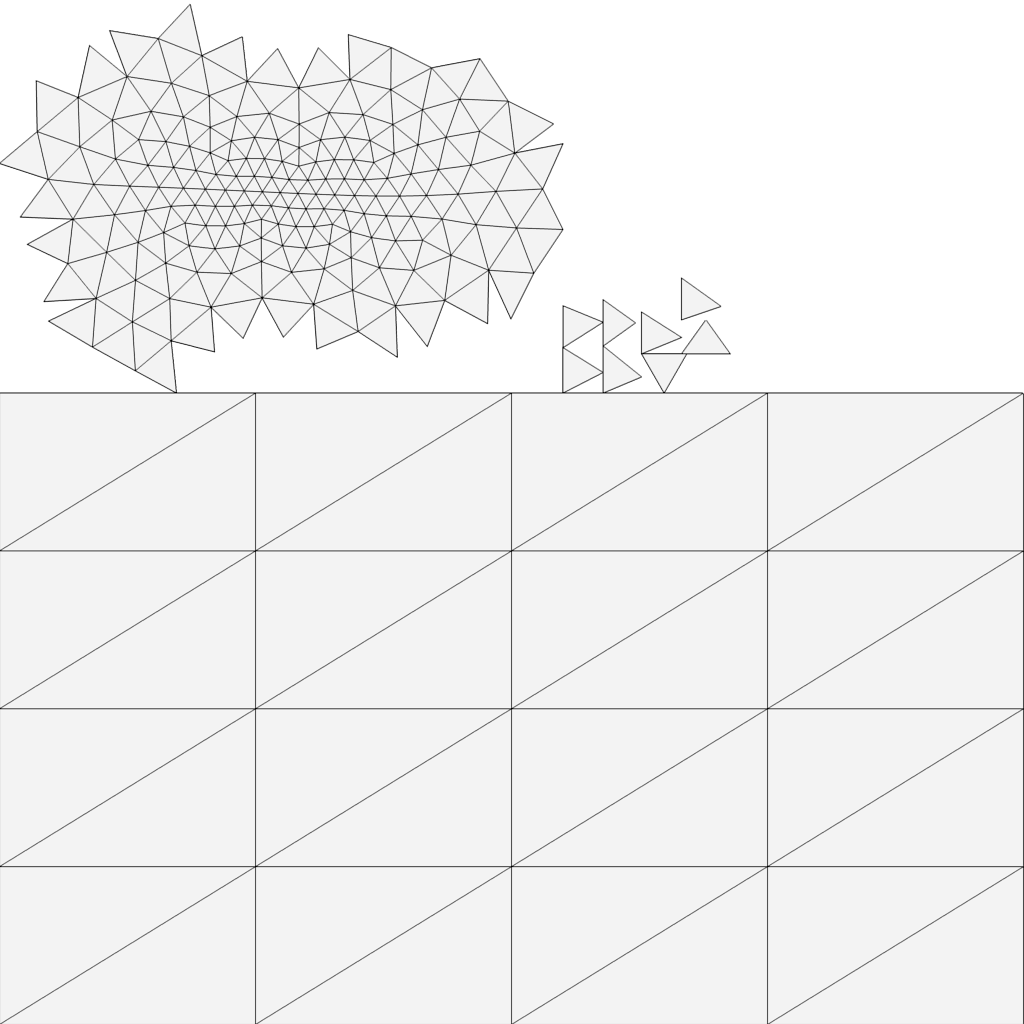
\includegraphics[scale=0.12]{images/state_of_art/unwrapping/prova_1.png}}\qquad\qquad
\subfigure[Smart UV Projects]{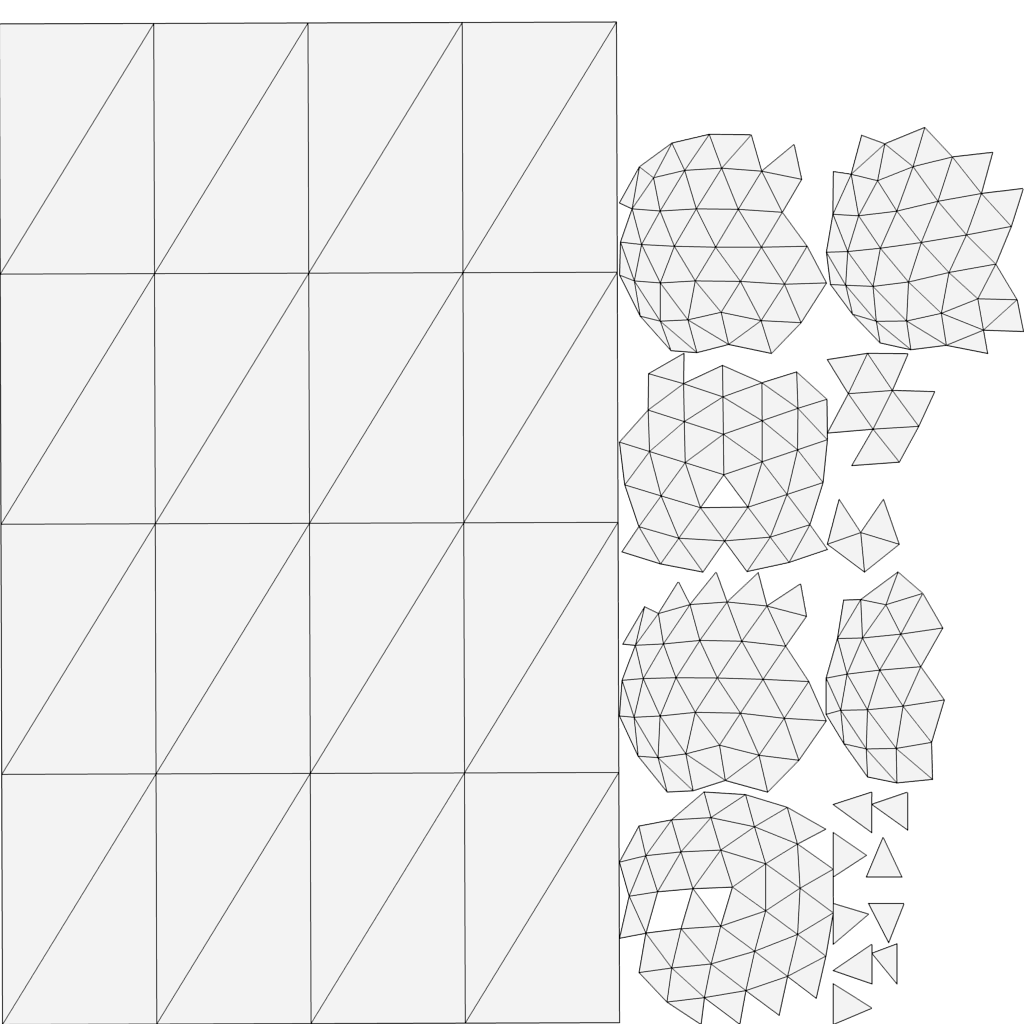
\includegraphics[scale=0.12]{images/state_of_art/unwrapping/prova_2.png}}\qquad\qquad
\caption{unwrapping per il modello prova.obj}
\label{img:soa_unwrapping_test}

\subfigure[Unwrapping]{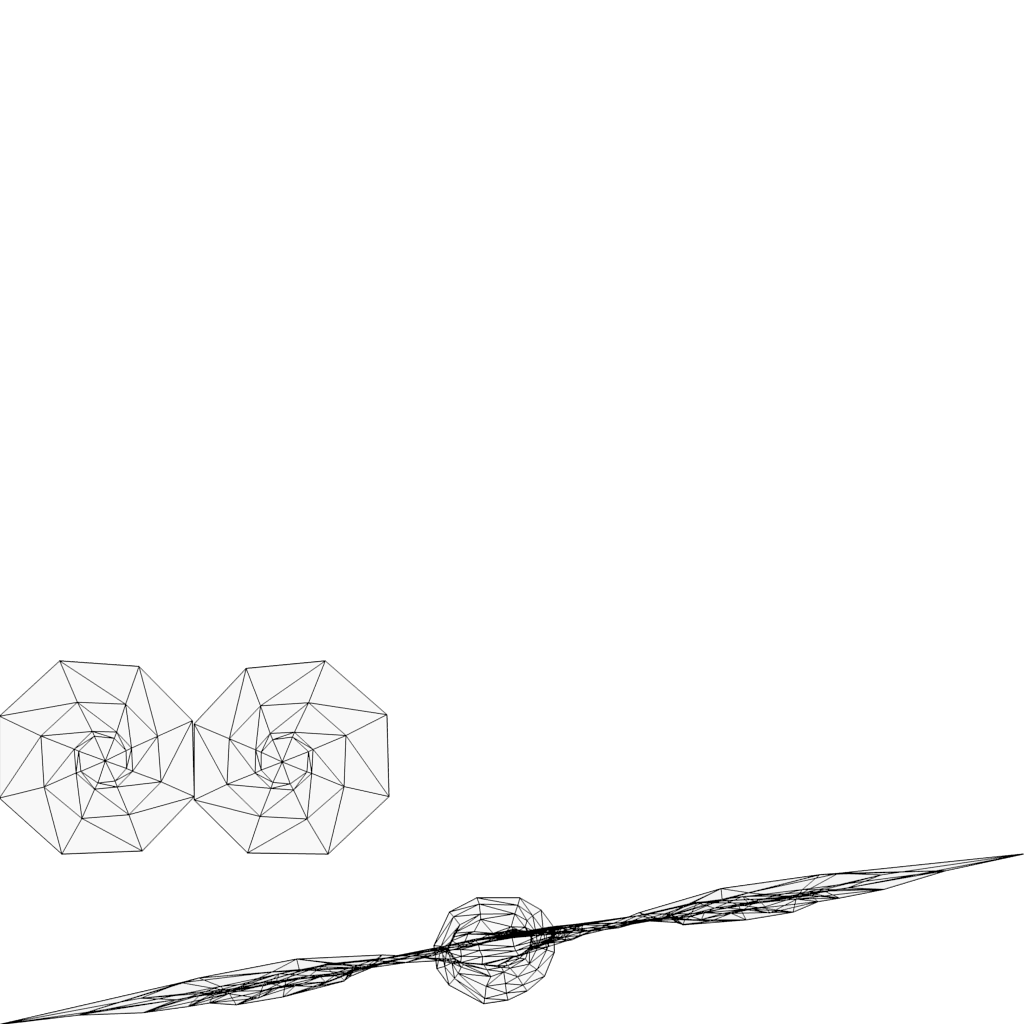
\includegraphics[scale=0.12]{images/state_of_art/unwrapping/monkey_1.png}}\qquad\qquad
\subfigure[Smart UV Projects]{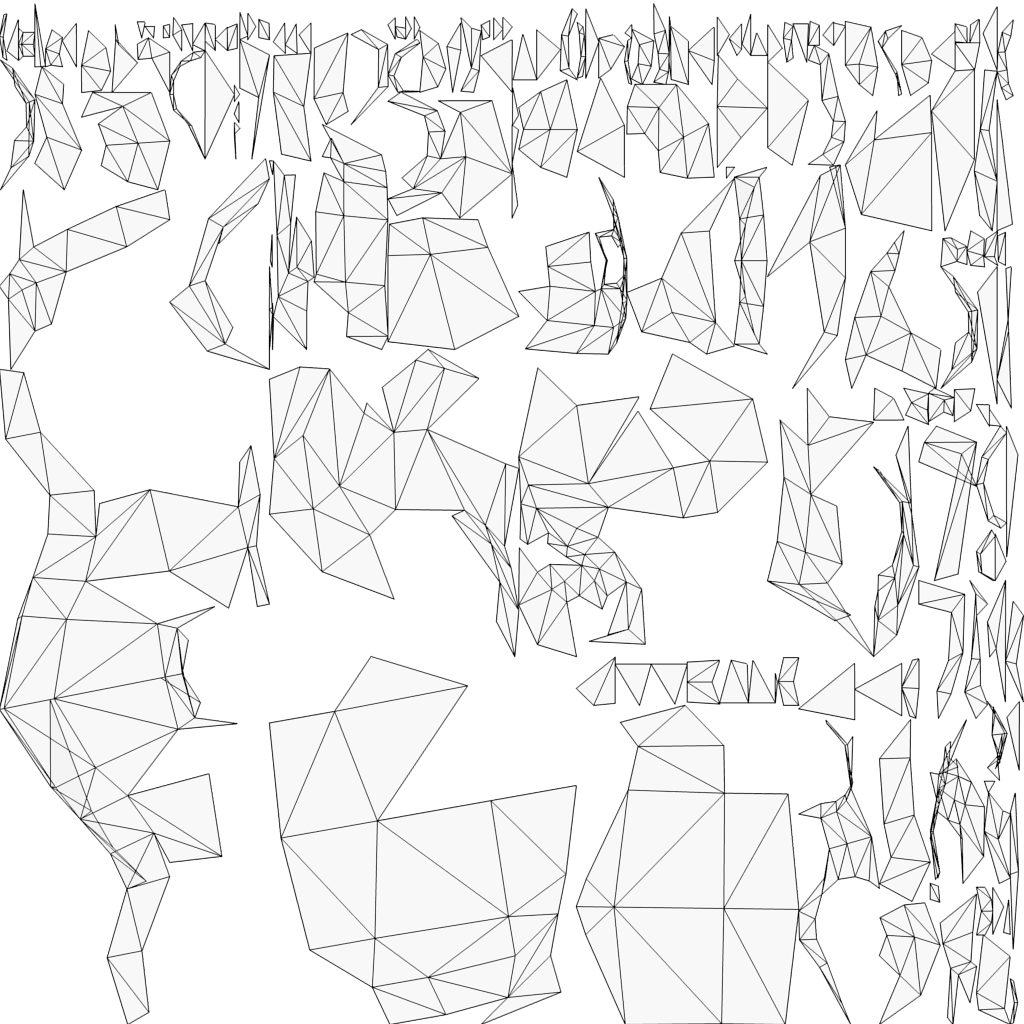
\includegraphics[scale=0.12]{images/state_of_art/unwrapping/monkey_2.png}}\qquad\qquad
\caption{unwrapping per il modello monkey.obj}
\label{img:soa_unwrapping_monkey}

\subfigure[Unwrapping]{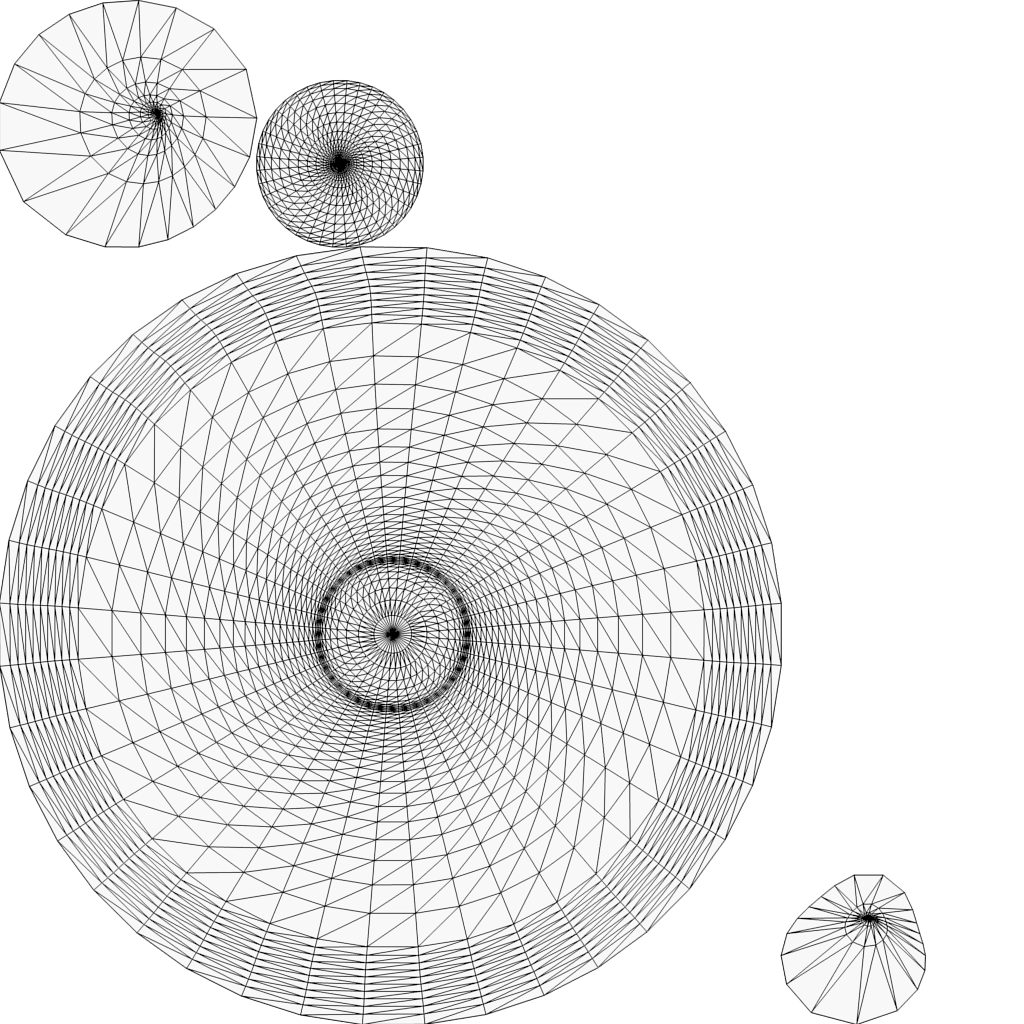
\includegraphics[scale=0.12]{images/state_of_art/unwrapping/teapot_1.png}}\qquad\qquad
\subfigure[Smart UV Projects]{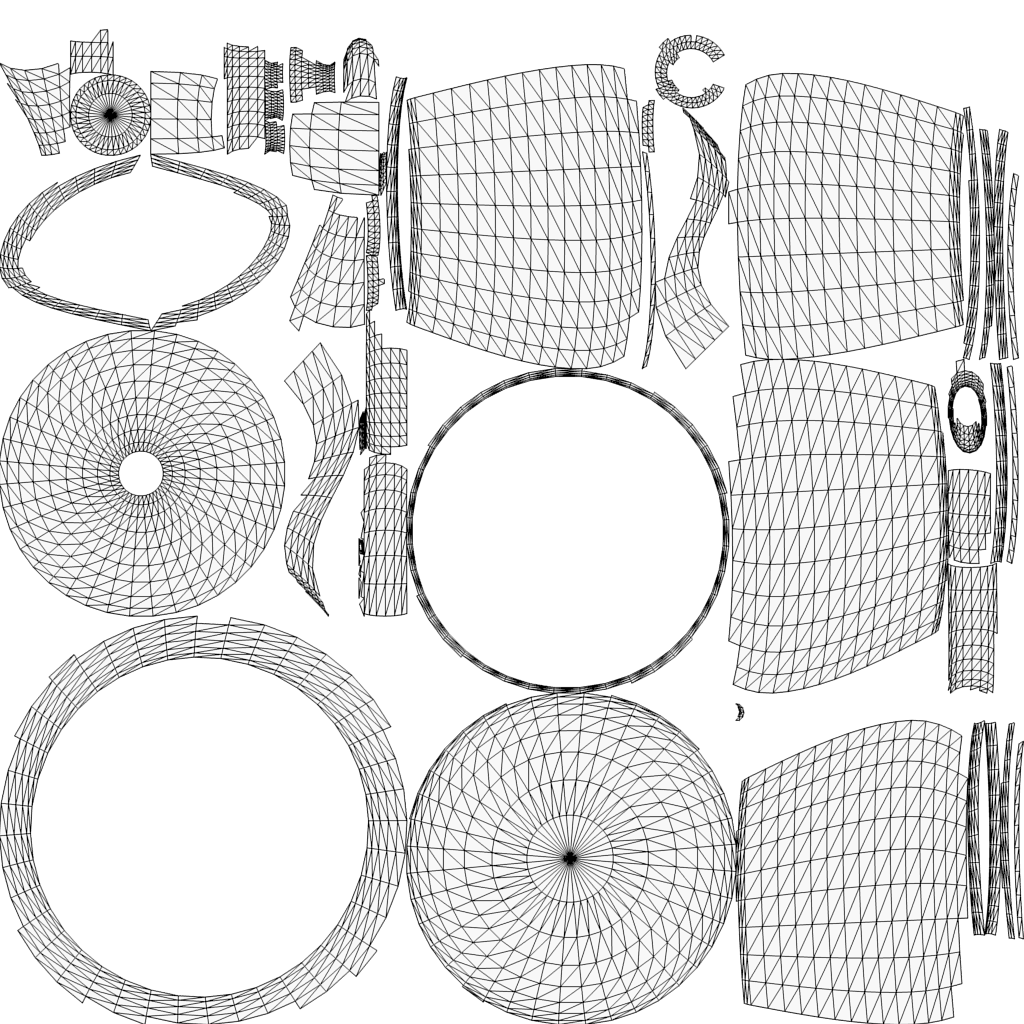
\includegraphics[scale=0.12]{images/state_of_art/unwrapping/teapot_2.png}}\qquad\qquad
\caption{unwrapping per il modello teapot.obj}
\label{img:soa_unwrapping_teapot}
\end{figure}

\subsection{Alcuni esempi}
I programmi di computer grafica 3D utilizzano l'unwrapping principalmente per il calcolo della mappa $UV$ (texture mapping). Lo spazio $UV$ viene utilizzato per la rappesentazione delle parametrizzazioni, � un sottospazio del piano $\mathbb{R}^2$ ed � definito da tutte le coppie di punti $(u,v)$ tali per cui $0<u<1$ e $0<v<1$. La mappa UV viene utilizzata per il texture mapping una tecnica che permette di applicare una immagine sopra una superficie, con lo scopo di conferire maggiori dettagli al modello.
% Magari era da mettere sopra.

Blender implementa varie tecniche che consentono di determinare una parametrizzazione per una generica superficie. Alcuni metodi di unwrapping sono automatizzati, mentre altre richiedono che l'utente fornisca delle informazioni iniziali (taglio sulla mesh). Le immagini \ref{img:soa_unwrapping_test}, \ref{img:soa_unwrapping_monkey} e \ref{img:soa_unwrapping_teapot} illustrano i risultati ottenuti in Blender utilizzando i metodi 'Unwrapping' e 'Smart UV Projects'.


% TODO \section{2D packing}

\section{Ambient occlusion}

L'ambient occlusion � un modello di riflessione locale della luce utilizzato per il calcolo dell'ombreggiatura. Contribuisce al conferimento di maggiore realismo ai modelli di illuminazione utilizzati nella computer grafica 3D. Il calcolo dell'ambient occlusion permette di ricavare l'attenuazione luminosa in ogni punto della geometria. Questo metodo globale fornisce un indice di illuminazione per ciascun punto, che � funzione della geometria della scena.

% Concetto sul calcolo dell'AO.
I metodi di calcolo dell'ambient occlusion si basano sulla visibilit� che la superficie ha dello sfondo. Per determinare l'indice di luminosit� di una superficie tridimensionale vengono tracciati dei raggi in ogni direzione dalla stessa. I raggi che intercettano un altro oggetto nella scena non contribuiscono alla luminosit� della superficie, mentre quelli che raggiungono lo sfondo n� aumentano l'illuminazione. Di conseguenza sar� possibile attribuire ad ogni punto della supericie un indice di illuminazione che si basa sul numero di raggi che raggiungono o meno lo sfondo della scena.

\section{Applicazioni}
Ha avuto successo nella produzione di animazioni grazie alla sua relativa semplicit� e efficienza. In gergo ambient occlusion viene chiamato anche "sky light". Una buona caratteristica di questo metodo di shading � quella di offrire una migliore percezione della forma tridimensionale degli oggetti mostrati. Questo fatto � riportato dai risultati di esperimenti che dimostrano la superiore resa della profondit� prodotta da uniforme illuminazione "sky light" diffusa rispetto alla "direct lighting". L'ambient occlusion � legata all'accessibility shading, che si basa sulla facilit� con cui un certo elemento (polvere, luce ecc...) pu� raggiungere ogni punto di una superficie (si pensi ad un oggetto poroso in cui i buchi meno accessibili tendono a rimanere coperti di polvere).

\subsection{Definizione del problema}
Data una superficie in forma cartesiana � possibile ricavare per ogni suo punto il valore dell'indice di luminosit� associato.Ipotizziamo di avere a disposizione l'equazione cartesiana che descrive la superficie $S$ orientabile $f(x,y) : D \subset \mathbb{R}^2 \rightarrow \mathbb{R}$, inoltre supponiamo che $f(x,y)$ sia differenziabile su tutti i punti interni a $D$.

Per ogni punto $P \in D$ � possibile quindi ricavare due piani tangenti alla superficie $S$ nel punto $A(P_x, P_y, f(P))$ e da questo determinare le normali $n(n_x, n_y, n_z)$ e $n'(-n_x, -n_y, -n_z)$. Dato che S � orientabile sar� possibile definire un campo vettoriale $n:S\subset \mathbb{R}^3 \rightarrow \mathbb{R}^3$ continuo che associa ad ogni punto $P$ della superficie la sua normale $n$. Da questo momento in poi ad ogni punto $A \in S$ associeremo un unico piano tangente $ \uppi $ 'orientato', definito come
\begin{displaymath}
\uppi: n_x x + n_y y + n_z z + d = 0
\end{displaymath}
con $n(A) = (n_x, n_y, n_z)$.
% Immagine del piano tangente

L'ambient occlusion in un punto $A(P_x, P_y, f(P))\in S$ pu� essere espresso in funzione della visibilit� che si ha dello sfondo dal punto di osservazione. Definiamo la funzione $V_A(\omega):\mathbb{R}^3 \rightarrow \mathbb{R}$ che esprime l'accessibilit� dello sfondo da parte del raggio che si origina dal punto $A$ e prosegue parallelamente a $\omega$ nello stesso verso.
\begin{displaymath}
V_A(\omega) = \left\{
\begin{array}{rl}
 0 & \mbox{se in direzione di $\omega$ il raggio non colpisce altre geometrie} \\ 
 1 & \mbox{altrimenti}
\end{array}
\right.
\end{displaymath}

Naturalmente i vettori $\omega$ che potranno contribuire direttamente all'aumento della luminosit� del punto sono solo quelli che si trovano sul semispazio positivo delimitato dal piano $\uppi$, cio� tutti quei $\omega$ tali per cui $\omega \cdot n > 1$. Inoltre vengono considerati solamente i vettori $\omega$ a norma unitaria, in definitiva $\omega$ potr� variare nell'insieme
$$ \Omega = \{ \omega \in \mathbb{R}^3 : \omega \cdot n > 0 \wedge \left\| \omega \right\| = 1 \} $$
L'insieme $\Omega$ definisce una semisfera giacente sul semipiano positivo di $\uppi$ e traslata nell'origine.

Abbiamo ora tutti i dati necessari a determinare l'indice di visibilit� associato al punto $A(P_x, P_y, f(P)) \in S$. L'occlusione pu� essere ricavata calcolando l'integrale di superficie di $V_a$ lungo la semisfera $\Omega$ rispetto all'angolo tra $n$ e $w$
$$ O(A) = \frac{1}{\uppi} \int\!\!\!\int_\Omega V_A(\omega)  (n \cdot \omega)  d\Omega $$
Il valore dell'integrale � massimo nel caso in cui per ogni $\omega \in \Omega, \; V_a(w) = 1$ e il suo valore � $2\uppi$, in questo caso il punto � completamente circondato da altre geometrie. Il valore minimo dell'integrale � 0 e si ha nel caso in cui il punto considerato abbia una visuale della scena completamente sgobra da altre goemetrie.

L'indice di luminosit� associato al punto $A$ pu� quindi essere ricavato in modo complementare dal valore dell'occlusione. Di conseguenza i punti della superficie circondati da molte altre geometrie otterrann� un basso indice di luminosit�, mentre i punti pi� liberi da ingombri risulteranno pi� luminosi.

\subsection{Ambient occlusion in pratica}
Nella pratica per approssimare questo integrale vengono utilizzate diverse tecniche, la pi� diretta � probabilmente quella che prevede l'uso del metodo Monte Carlo per tracciare raggi dal punto $A$ e valutare le intersezioni con la geometria della scena. (ray casting). Un altro approccio (pi� adeguato per l'accelerazione hardware) � quello di rasterizzare le geometrie viste dal punto $A$ (a cui viene assegnato il colore nero) in confronto allo sfondo (a cui viene assegnato il colore bianco) e poi prendere in considerazione una media ponderata delle porzioni rasterizzate. Quest'ultimo metodo � un esempio di approccio "inside-out" (o "gathering"), mentre altri algoritmi (come la depth-map ambient occlusion) utilizzano tecniche di "scattering" o "outside-in".

Nel nostro programma l'ambient occlusion viene calcolato utilizzando un approccio 'inside-out'. La geometria viene suddivisa in un insieme di triangoli, utilizzando un processo di triangolizzazione della mesh. Ogni triangolo $T$ viene quindi discretizzato in un insieme di punti $P_t$, per ciascuno di essi viene renderizzata la scena visibile dal punto in direzione della normale alla superficie $T$. Le geometrie visibili saranno rasterizzate nel buffer video con un colore nero, mentre allo sfondo sar� assegnato il colore bianco. L'occlusione $O(A$) sar� quindi calcolata come media pesata dei singoli contributi in pixel della texture. Da questo valore sar� possibili determinare la luminosit� associata al punto $P_t$ del triangolo $T$.

\subsection{Alcuni esempi}

L'ambient occlusion conferisce maggiore realismo all'illuminazione di una scena. Questa tecnica � ampiamente diffusa nei programmi di elaborazione tridimensionale e non solo, viene utilizzata anche nei videogiochi e nei simulatori di realt� virtuale. Una versione real time per il calcolo dell'ambient occlusion viene utilizzata per il rendering in tempo reale (ad esempio nei videogiochi) ed � chiamata Screen Space Ambient Occlusion (SSAO). Il calcolo dell'ambient occlusion lo troviamo implementato in Blender attraverso l'uso di un metodo statistico non parametrico e del ray casting. 

\subsubsection{Blender}
Vediamo ora come si utilizza il calcolo dell'ambient occlusion in blender. I settaggi dell'ambient occlusion si trovano nel pannello Shading, una sottovoce del pannello World. Per default l'ambient occlusion � inattivo, se viene attivato, nel pannello appaiono le relative opzioni (\figurename~\ref{fig:soa_ao_blender}).

\begin{figure}[!h]
\centering %
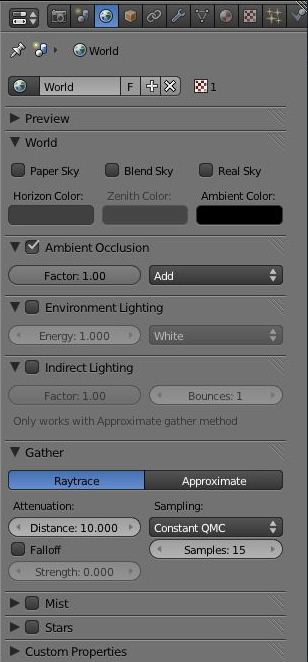
\includegraphics[scale=0.3]{images/state_of_art/ao/blender/ao.jpg}
\caption{configurazione dell'ambient occlusion in Blender 2.57.1 \label{fig:soa_ao_blender}}
\end{figure}

Blender utilizza il ray casting per il calcolo dell'occlusione associato a un punto della geometria. I raggi sono inviati all'emisfero secondo una distribuzione casuale fino a che il numero di raggi emessi � sufficientemente elevato da fornire buoni dati statistici,  questo causa differenze sensibili nel pattern di occlusione dei pixel circostanti. Ecco perch� il calcolo dell'AO genere immagini con grana, che appaiono un po sporche se non ci sono abbastanza raggi. Il numero di raggi emessi � controllato dal pulsante numerico Samples (campionamenti). Il valore di default 5 � generalmente adatto a generare anteprime, il reale numero di raggi emessi � questo valore al quadrato. Ovviamente anche i tempi di rendering aumentano con l'aumentare del numero dei campionamenti.

\begin{figure}[!htpb]
\centering %
\subfigure[1 campione]{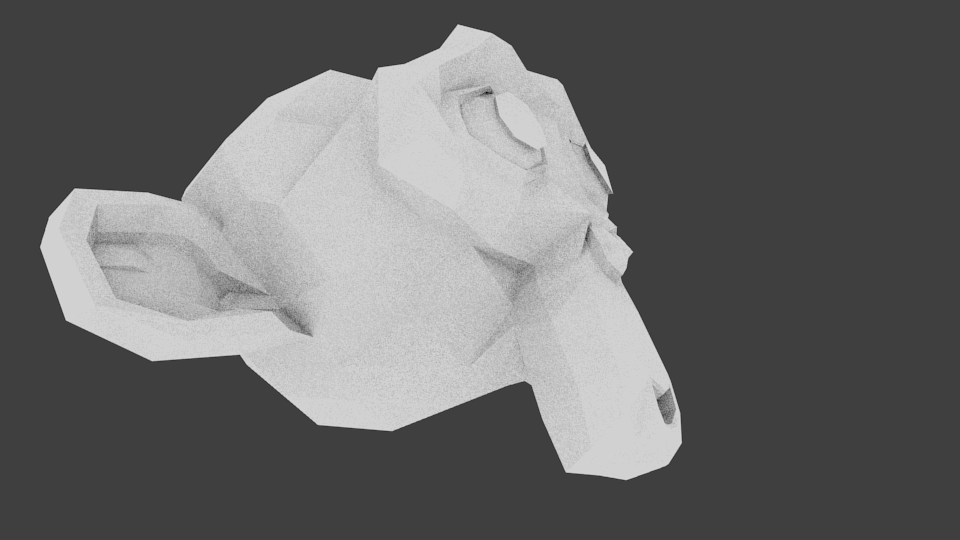
\includegraphics[scale=0.13]{images/state_of_art/ao/blender/monkey_ray_1sample.png}}\qquad
\subfigure[25 campioni]{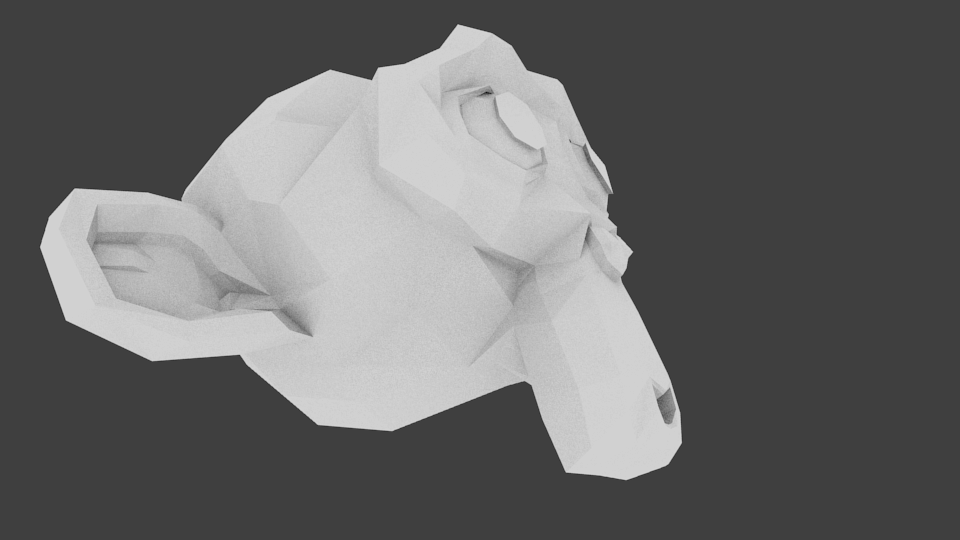
\includegraphics[scale=0.13]{images/state_of_art/ao/blender/monkey_ray_5sample.png}}\qquad
\subfigure[100 campioni]{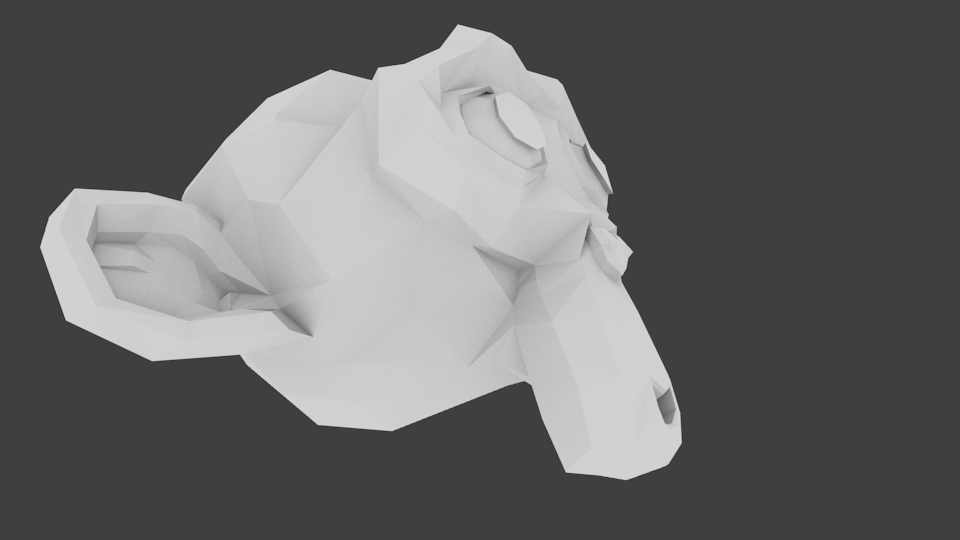
\includegraphics[scale=0.13]{images/state_of_art/ao/blender/monkey_ray_10sample.png}}\qquad
\caption{ambient occlusion per il modello monkey.obj}

\subfigure[1 campione]{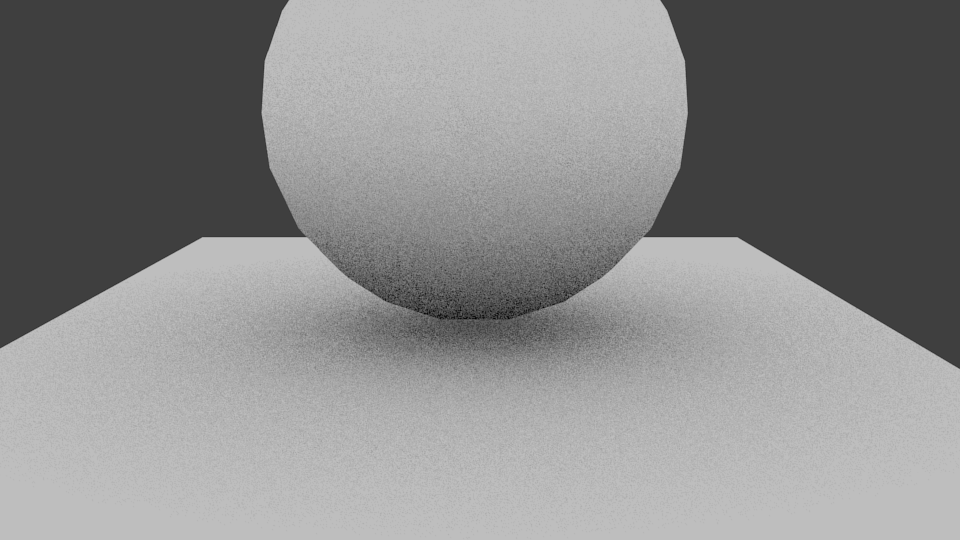
\includegraphics[scale=0.13]{images/state_of_art/ao/blender/prova_ray_1sample.png}}\qquad
\subfigure[25 campioni]{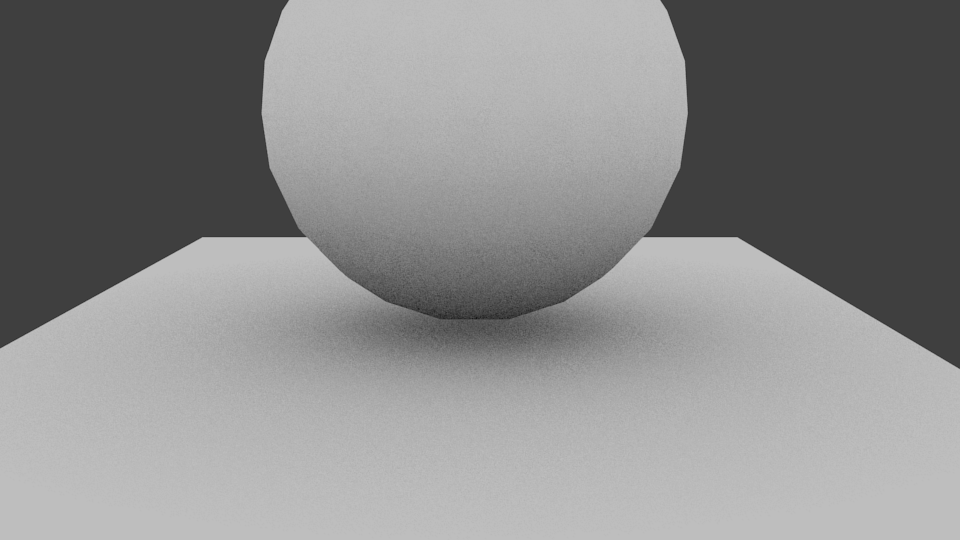
\includegraphics[scale=0.13]{images/state_of_art/ao/blender/prova_ray_5sample.png}}\qquad
\subfigure[100 campioni]{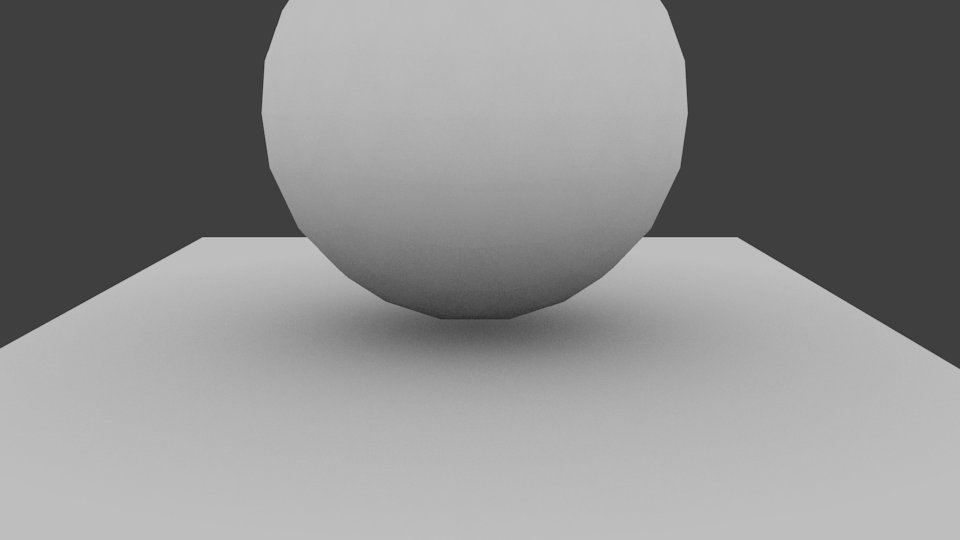
\includegraphics[scale=0.13]{images/state_of_art/ao/blender/prova_ray_10sample.png}}\qquad
\caption{ambient occlusion per il modello prova.obj}

\subfigure[1 campione]{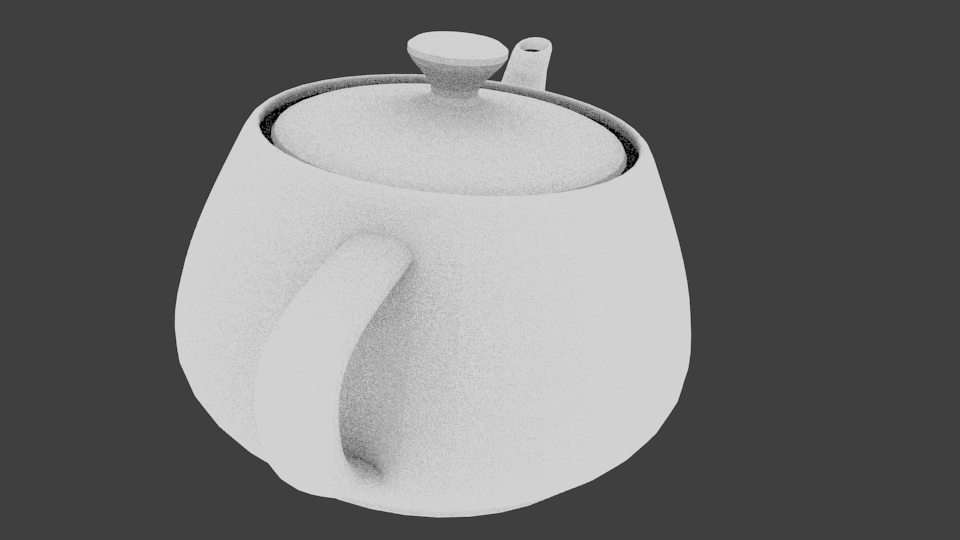
\includegraphics[scale=0.13]{images/state_of_art/ao/blender/teapot_ray_1sample.png}}\qquad
\subfigure[25 campioni]{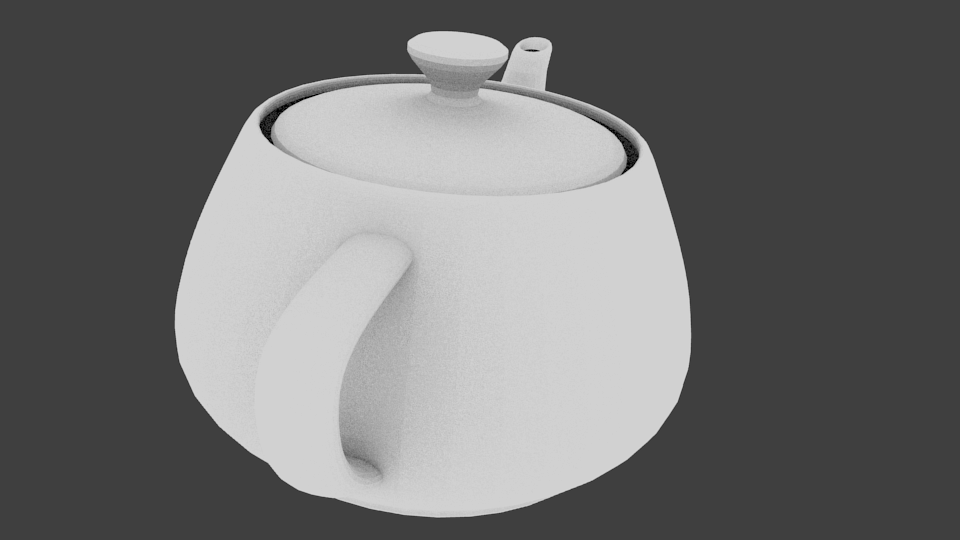
\includegraphics[scale=0.13]{images/state_of_art/ao/blender/teapot_ray_5sample.png}}\qquad
\subfigure[100 campioni]{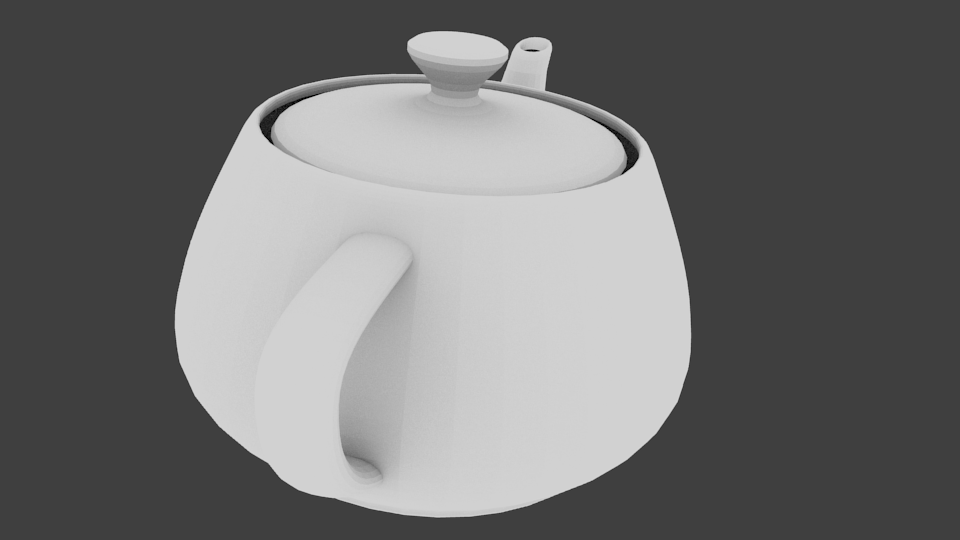
\includegraphics[scale=0.13]{images/state_of_art/ao/blender/teapot_ray_10sample.png}}\qquad
\caption{ambient occlusion per il modello teapot.obj}
\end{figure}


\chapter{Sviluppo del progetto}

\section{Ambiente di sviluppo}

Lo sviluppo del progetto � stato portato avanti in ambiente Windows. Il programma � stato pensato per essere eseguito su macchine Windows senza la necessit� di intervento umano. Microsoft Visual Studio 2005 � l'ambiente di sviluppo utilizzato per la programmazione e il debug dell'applicativo. La scelta del linguaggio di implementazione � ricaduta sul C++, questa scelta � stata dettata pi� che altro da questioni di compatibilit� con altri software sviluppati dalla Seac02, ma anche dalla possibilit� di realizzare un codice a oggetti di facile lettura e modulare.

% Si potrebbe parlare di Visual Studio 2005?

Oltre ai classici strumenti per la programmazione � stato utilizzato SVN un applicativo per il software versioning del codice. Il software versioning � il processo di assegnazione di un nome di versione (o numero di versione) univoco a un univoco stato dell'applicativo in fase di sviluppo. SVN Subversion � un programma per il controllo delle revision chei permette di tenere traccia della differenze incrementali tra diverse versioni del progetto, inoltre consente l'accesso concorrente da parte di un team di sviluppo. SVN � realizzato con un modello client-server, la traccia del progetto � memorizzata lato server e l'utente pu� richiedere varie operazioni da eseguire su una determinata versione del progetto.

\subsection{Librerie di supporto}
L'applicativo si basa sull'utilizzo di alcune librerie esterne tra cui Qt, OpenSG e IpOpt. QT � stato utilizzato per la realizzazione del front-end dell'applicativo e come ambiente per ospitare OpenSG. Una versione modificata di OpenSG � utilizzato come gestore scenografico per la creazione di un contesto operativo per la grafica tridimensionale. IpOpt fornisce una serie di routine per la risoluzione di problemi di minimizzazione non lineari, � utilizzato per il processo di unwrapping automatico.

Qt � una libreria multipiattaforma per lo sviluppo di programmi con interfaccia grafica tramite l'uso di widget. Qt, ampiamente utilizzato nell'ambiente desktop KDE, viene sviluppato dall'azienda Qt Software. Qt usa il linguaggio C++ standard con un estensivo uso del preprocessore C per arricchire il linguaggio, ma esistono interfacce per Java, Python, C, Perl e PHP. Gira sulle piattaforme principali ed integra funzioni per l'accesso ai database SQL, parsing di documenti XML ed API multipiattaforma per l'uso dei file. 

OpenSG � un framework basato su OpenGL per la realizzazione di un sistema scenografico creato per programmi di grafica real-time. OpenSG � sviluppato seguendo i principi dei software Open Source, � distribuito sotto licenza LGPL pu� quindi essere usato gratuitamente. La compatibilit� � garantita con i sistemi Microsoft Windows, Linux, Solaris e Mac OS X. Tra le principali caratteristiche c'� il supporto avanzato alla programmazione multithreading e al calcolo distribuito, anche se � perfettamente utilizzabile su una singola macchina in single-thread.

% [possibile sviluppo - modello software versioning utilizzato, + cose su SVN]

% [possibile sviluppo - convenzioni sul lavoro - doxygen]

\subsection{Richieste hardware}
L'unica richiesta hardware per l'uso del programma � che la scheda video abbia i framebuffer. Il framebuffer � una memoria della scheda video nella quale vengono memorizzate le informazioni destinate all'output per la rappresentazione di un intero fotogramma sullo schermo, sono contenute le informazioni sul colore di ciascun pixel. Le dimensioni del framebuffer dipendono dalla risoluzione dell'output video e dalla profondit� di colore. Il framebuffer � utilizzato nell'applicativo per il calcolo dell'ambient occlusion, in particolare vengono utilizzati i risultati delle renderizzazioni della scena memorizzati nel buffer.

% Naming convection

\section{Lavoro precedente}

Il lavoro fin qui svolto � stato gi� ottenuto da sviluppi precedenti. Proseguiremo ora con la valutazione dei risultati gi� acquisiti, discutendo se questi rispondono alle nostre necessit�. In base a queste valutazioni determineremo i punti critici dell'applicativo e procederemo di conseguenza per ciascuno. Alcune valutazioni porteranno a una completa riconsiderazione dell'approccio seguito, mentre altri richiederanno solamente una ristrutturazione di quello gi� ottenuto. Prima dei testi di valutazione descriveremo a grandi linee i principi di funzionamento del programma, discutendo sulle principali fasi che intercorrono per il calcolo della scena in output.

\subsection{Obiettivi}
L'obiettivo � quello di realizzare un programma in grado di calcolare l'ambient occlusion delle geometrie di una scena.
L'ambient occlusion di ciascuna geometria dovr� essere rappresentata su di una texture che verr� applicata come materiale sulla geometria stessa. Come risultato si vuole ottenere una scena nello stesso formato di quella data con in pi� applicate le varie texture dell'ambient occlusion calcolate. Il programma si trova gi� in fase di sviluppo sar� quindi necessario prima fare il punto della situazione ed analizzare i risultati fin qui ottenuti, per poi determinare i passi successivi nella sua realizzazione.


\subsection{Struttura del programma} \label{subsez:program_struct}
Il programma si basa su un principio molto semplice che ne garantisce il funzionamento con qualsiasi scena in ingresso. Il fondamento su cui si basa � il considerare ciascuna
geometria della scena data in ingresso come composta da un insieme di triangoli. Le fasi successive vengono portate avanti seguendo un approccio orientato ai triangoli,
in questo modo si pu� semplificare il calcolo della parametrizzazione $UV$ della geometria � il packing dei triangoli nella texture. Mentre il calcolo dell'ambient occlusion non
trae particolari vantaggi da questo approccio.

Nella fase preparatoria vengono estratti tutti i nodi geometrie dalla scena data in ingresso. OpenSG organizza la scena in ingresso in una struttura dati ad albero composta
da una serie di nodi differenti (per la geometria, l'illuminazione, le trasformazioni, ecc ...). Gli unici nodi di nostro interesse sono quelli di trasformazione e di geometria,
i primi memorizzano le trasformazioni effettuate sulla scena (a partire da quel nodo in poi) mentre i secondi sono i nodi che contengono la struttura dati della mesh.
L'importanza dei nodi di trasformazione � da ritrovarsi nel fatto che � necessario ricostruire la scena in uscita come si presentava in ingresso, se non si considerasse
allora la scena in uscita verrebb� ricostruita in modo errato. I nodi di trasformazione non vengono gestiti direttamente ma ne vengono considerati solo gli effetti attraverso
un metodo richiamabile da ciascuna geometria. All'interno di ciascun nodo geometria � contenuta una struttura dati di OpenSG per la memorizzazione della mesh, per
ciascuno di essi verranno eseguite le fasi che andremo ora a descrivere.

\subsubsection{Prima fase}
OpenSG memorizza la geometria in una struttura dati personalizzata che implementa la memorizzazione face-vertex di mesh. Vengono memorizzate due list una per le facce che compongono le geometrie e l'altra per i vertici associati.% [esempio]
Le informazioni legate a ciascun vertice possono essere memorizzate in tre modalit� differenti. La prima � la memorizzazione senza indici, in questo modo ciascun vertice di ciascuna facce replica in memorie le proprie informazioni (posizione, normale, colore, ecc ...).  La seconda � la memorizzazione a singola indicizzazione, in questo caso un vertice pu� fare riferimento a dati appartenenti ad un altro vertice. L'ultimo tipo � la memorizzazione a indici multipli, differisce dalla precedente dal fatto che il vertice pu� fare riferimento ai singoli dati di pi� vertici. Nell'immagine \ref{img:opensg_indexing} si pu� vedere un riepilogo delle tre modalit� di gestione dei dati associati ai vertici.

\begin{figure}[!htb]
\centering %
\subfigure[senza indici]{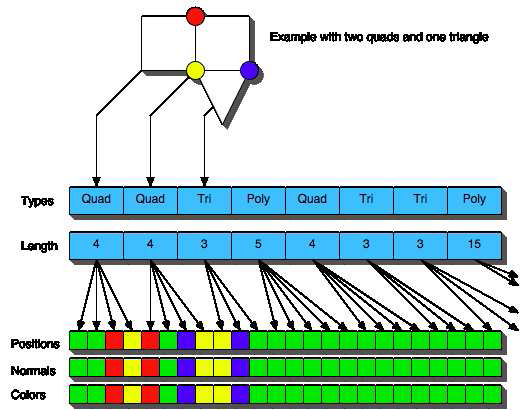
\includegraphics[scale=0.3]{images/previously_work/opensg/no_index.png}}\qquad
\subfigure[indici semplici]{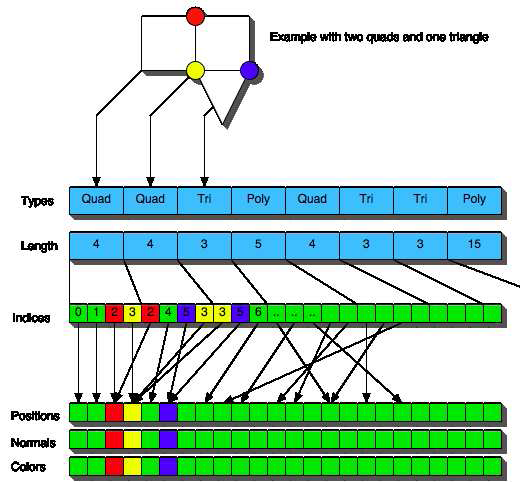
\includegraphics[scale=0.3]{images/previously_work/opensg/index.png}}\qquad
\subfigure[multi indice]{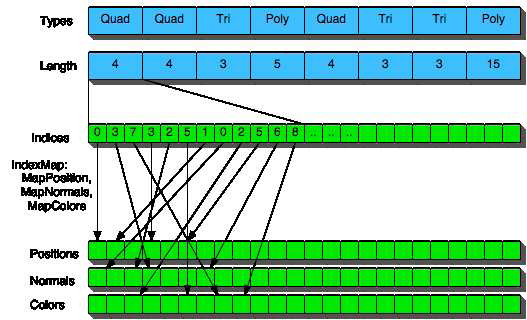
\includegraphics[scale=0.3]{images/previously_work/opensg/multi_index.png}}
\caption{riepilogo delle modalit� di memorizzazione}
\label{img:opensg_indexing}
\end{figure}

OpenSG mette a disposizione una serie di metodi che permettono di accedere alle singole facce che compongono la geoemtria (triangoli, rettangoli, poligoni, ecc ...), in particolare il metodo Triangle Iterator permette di iterare su ogni triangolo. Questi metodi vengono utilizzati dall'applicativo per l'accesso alla struttura dati della mesh.

Il programma richiede che ogni geometria memorizzi le informazioni per ciascun vertice in modo separato. Il motivo � che durante la fase di parametrizzazione � necessario che ogni vertice possa memorizzare informazioni differenti in funzione della faccia presa in considerazione. Infatti, nello spazio $O_{uv}$, pu� capitare che un vertice assumi posizioni differenti in funzione del triangolo a cui fa' riferimento, per questo motivo � necessario salvare differenti coordinate di texture per ogni vertice e per ogni faccia. Per questo motivo nella prima fase la geometria viene convertit� in modalit� di memorizzazione senza indici.

\subsubsection{Seconda fase}
Nella seconda fase avviene la parametrizzazione della superficie e il packing delle aree ottenute in $O_{uv}$. Per prima cosa ogni triangolo della geometria viene inserito in una classe contenitore ZedAOFaceInfoBuilder che ne calcola le coordinate bidimensionali, queste si otterranno banalmente per proiezione sul piano con normale pari a quella del triangolo considerato. Ogni triangolo viene successivemente traslato in $O_{uv}$ in modo tale che non vi siano coordinate negative.

%[immagine che ne spiega il processo.]

Si passa successivamente al packing delle superfici parametrizzate in $O_{uv}$. Viene quindi instaziato un oggetto della classe ZedAOTextureBoxPacker che si occupa di effettuare il packing delle aree. L'algoritmo utilizzato per il packing segue un approccio greedy per determinare una possibile disposizione dei triangoli su un quadrato. I triangoli vengono ordinati per valore di area decrescente, quindi prosegue con il packing di ciascun triangolo all'interno del quadrato. Il packing procede per traslazioni successive nelle direzioni di $u$ e $v$, fino a quando trova la prima traslazione che non si sovvrappone con i triangoli gi� inseriti. Durante la fase di packing a ciascun triangolo vengono assegnate le coordinate di texture definitive conformi dalle specifiche che definiremo pi� avanti

\subsubsection{Terza fase}
Nella terza ed ultima fase vengono calcolati i texel associati ai triangoli e viene generata la texture dell'ambient occlusion. Intuitivamente i texel associati a un triangolo possono essere definiti come i pixel occupati sull'area UV della texture. I texel vengono calcolati a partire dalle coordinate $UV$ associate ai vertici del triangolo, si procede per costruzione verticale. Si determinano i valori $U_{min}$ e $U_{max}$ tra cui variare con passo equivalente di un pixel, per ogni valore di $U$ si calcolano i valori $V_{min}$ e $V_{max}$, si crea quindi il texel associato le coordinate in pixel corrispondenti al valore attuale di $U$ e $V$ (immagine x). Per ogni texel vengono memorizzate alcune informazioni tra le pi� rilevanti: il valore delle normale, le
coordinate $XY$ in pixel e le coordinate $UV.$

Dopo aver determinato i texel che compongono la texture si procede con il calcolo dell'ambient occlusion. Per ogni texel della texture si effettua la renderizzazione della scena vista dalla posizione attuale in direzione e verso della normale del triangolo associato al texel. Si otterr� quindi una immagine della visuale che si ha della scena dalla posizione attuale, in base a questa verr� calcolata la gradazione di grigio da associare al pixel

\subsection{Test sulle mesh di prova}
Eseguiremo ora una serie di test di valutazione del programma su alcune mesh di prova. Prenderemo quindi in considerazione gli output delle varie fasi e da questi valuteremo
gli eventuali problemi. Successivamente procederemo con l'analisi delle problematiche riscontrate e la discussione su come risolverle.

\begin{figure}[!b]
\centering %
\subfigure[packing]{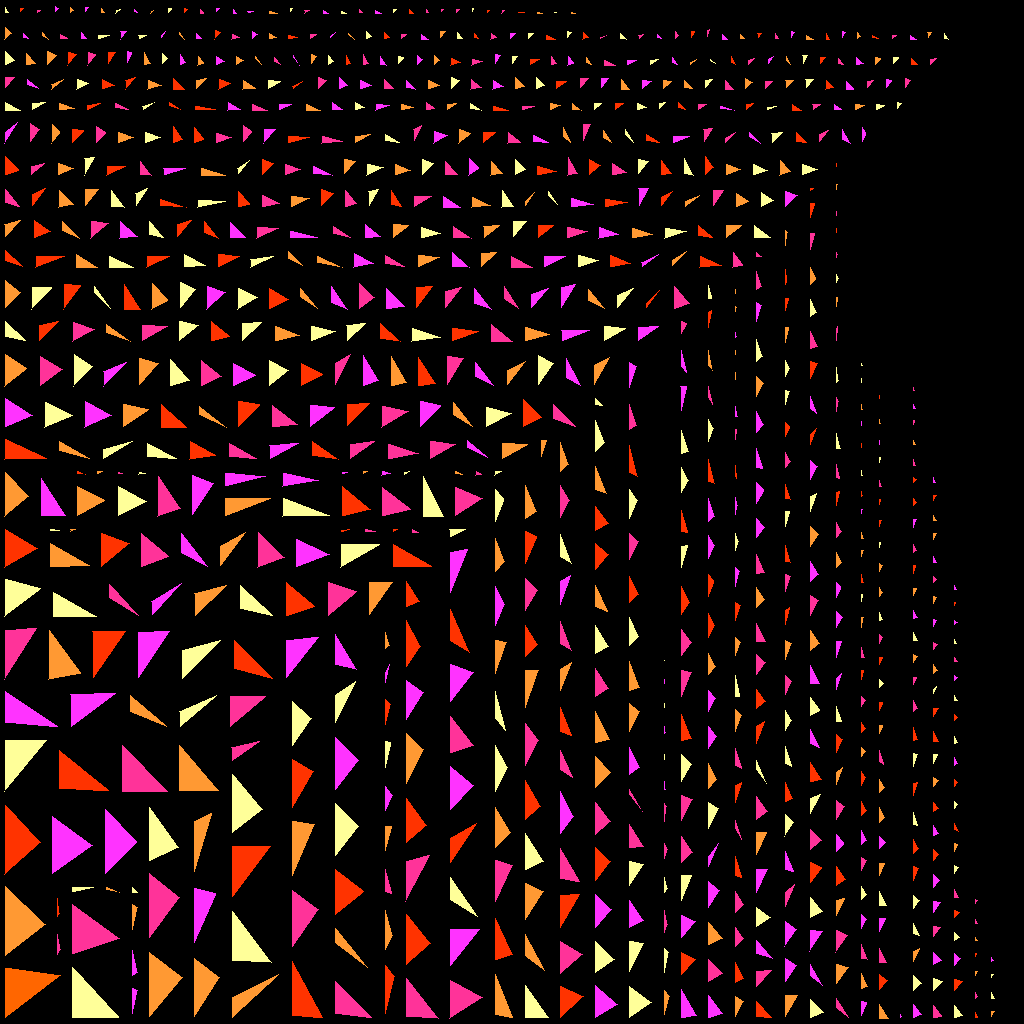
\includegraphics[scale=0.12]{images/previously_work/monkey/texel_dump.png} \label{img:test_monkey_partial_1}}\qquad
\subfigure[AO texture]{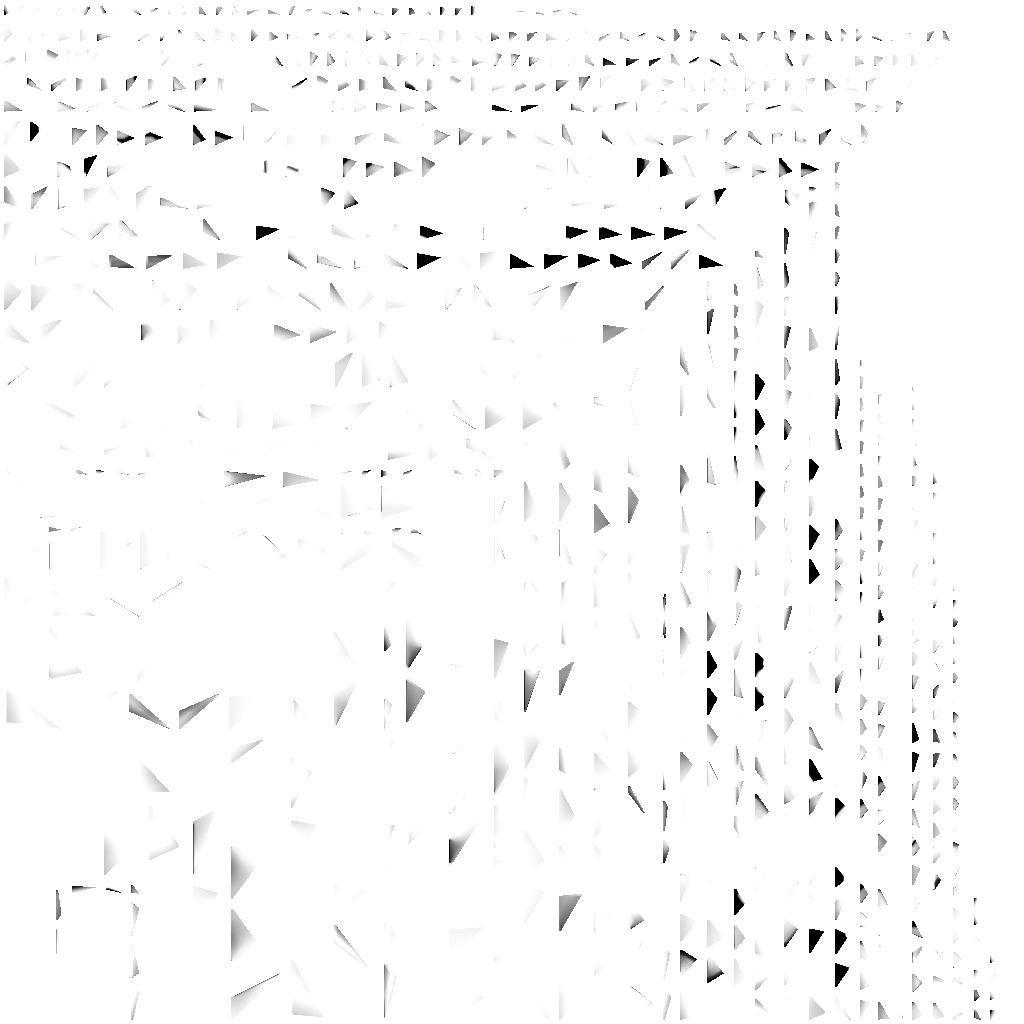
\includegraphics[scale=0.12]{images/previously_work/monkey/texture.png} \label{img:test_monkey_partial_2}}\qquad
\caption{output delle fasi intermedie per il modello monkey.obj}
\label{img:test_monkey_partial}
\end{figure}

\subsubsection{Test con il modello monkey.obj}
Prendiamo in considerazione il modello della scimmia monkey.obj, generato con l'aiuto di Blender. L'immagine \ref{img:test_monkey_partial_1} rappresenta l'output della disposizione dei triangoli all'interno della texture, da questa non si riscontrano particolari problemi. La texture dell'ambient occlusion � rappresentata sull'immagine \ref{img:test_monkey_partial_2}, anche in questo caso non si osservano particolari problematiche.

Per determinare il risultato finale utilizziamo i vari output del programma in combinazione con Blender. La scena in uscita in formato obj viene utilizzato come modello per l'applicazione della texture, infatti, questa contiene le coordinate $UV$ calcolate nel programma. Nell'immagine \ref{img:test_monket_out} si pu� osservare il risultato dell'applicazione della texture sul modello con disattivati tutti i filtri, per poterne osservare il risultato dell'applicazione diretta senza alterazioni.

\begin{figure}[!htpb]
\centering %
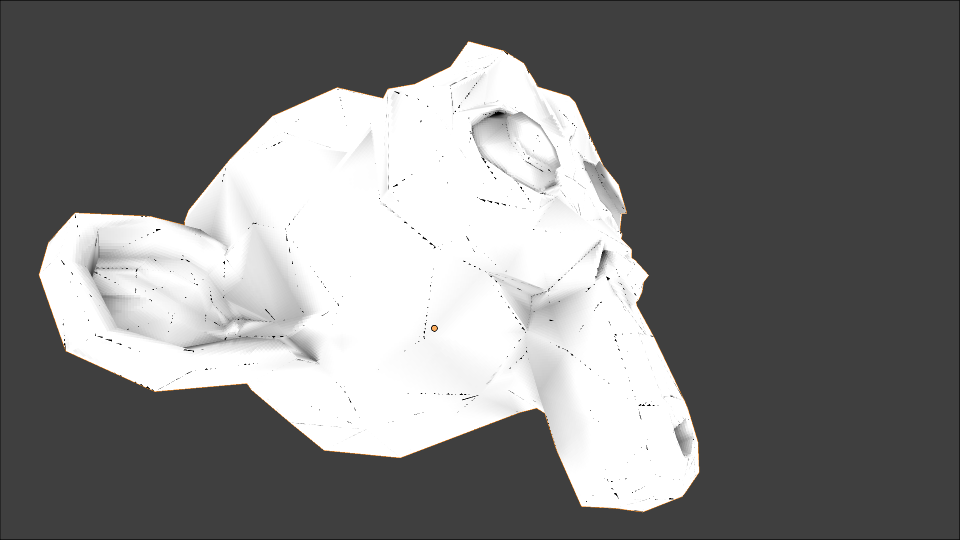
\includegraphics[scale=0.3]{images/previously_work/monkey/final_output.png}
\caption{output del modello monkey.obj}
\label{img:test_monket_out}
\end{figure}

L'applicazione della texture mette in rilievo alcuni problemi che finora non si erano presentati. Confrontando con l'AO calcolato da Blender si pu� facilmente osservare che
il risultato ottenuto non � certamente quello desiderato. Nelle immagini \ref{test_monkey_det_1} e \ref{test_monkey_det_2} si possono osservare due dettagli della scena, nella prima si osservano degli spazi neri in cui non � presenta la texture, nella seconda si osservano le diverse orientazioni dei pixel tra superfici adiacenti.
\begin{figure}[!htpb]
\centering %
\subfigure[tagli]{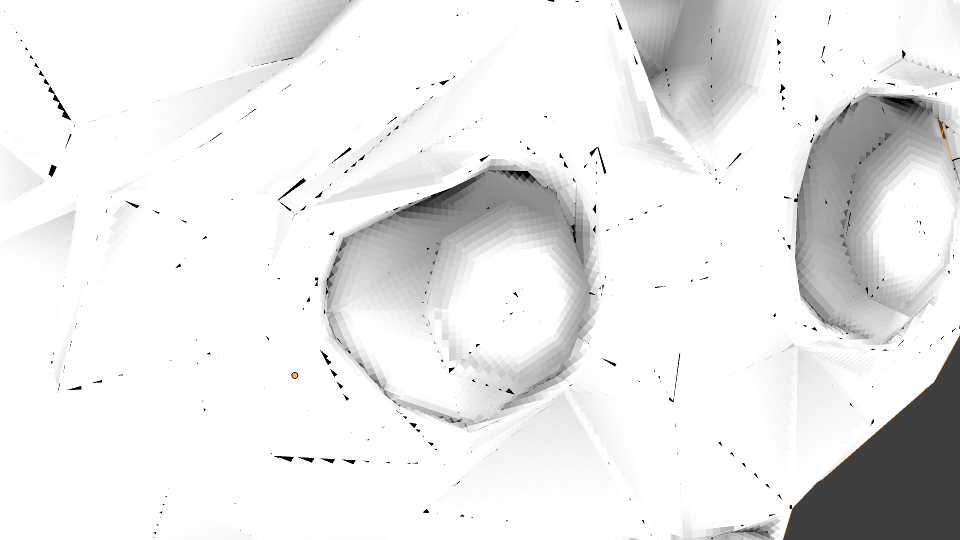
\includegraphics[scale=0.20]{images/previously_work/monkey/cuts.png} \label{test_monkey_det_1}}\qquad
\subfigure[discontinuit�]{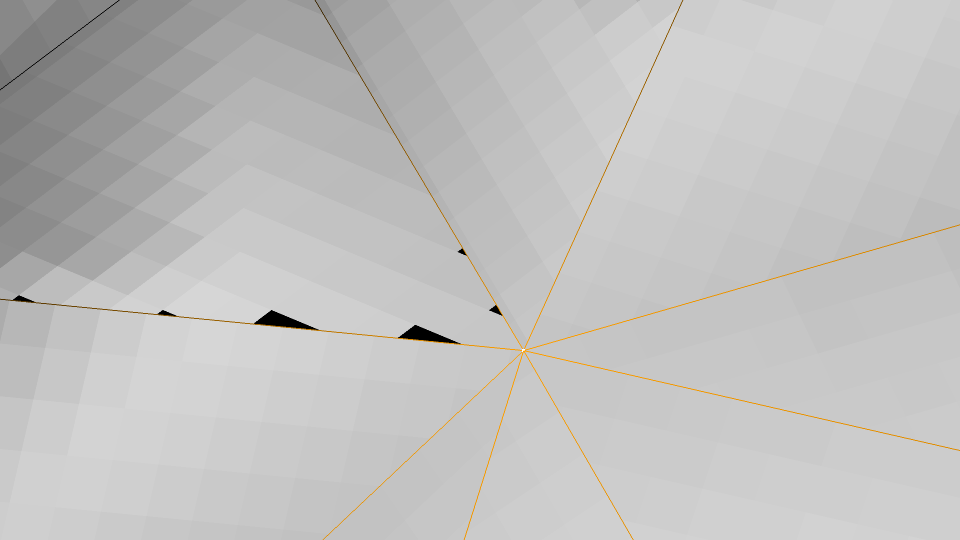
\includegraphics[scale=0.20]{images/previously_work/monkey/discontinuity.png} \label{test_monkey_det_2}}
\caption{dettagli relativi al modello monkey.obj}
\end{figure}

\subsubsection{Test con il modello teapot.obj e il modello prova.obj}
Verifichiamo ora che i problemi riscontrati con il modello monkey.obj si ripresentano con altri modelli. Le immagini \ref{img:test_teapot} e \ref{img:test_prova} rappresentano gli output delle varie
fasi di esecuzione del programma, la prima del packing e la seconda del calcolo dell'AO Texture.

\begin{figure}[!htb]
\centering %
\subfigure[packing]{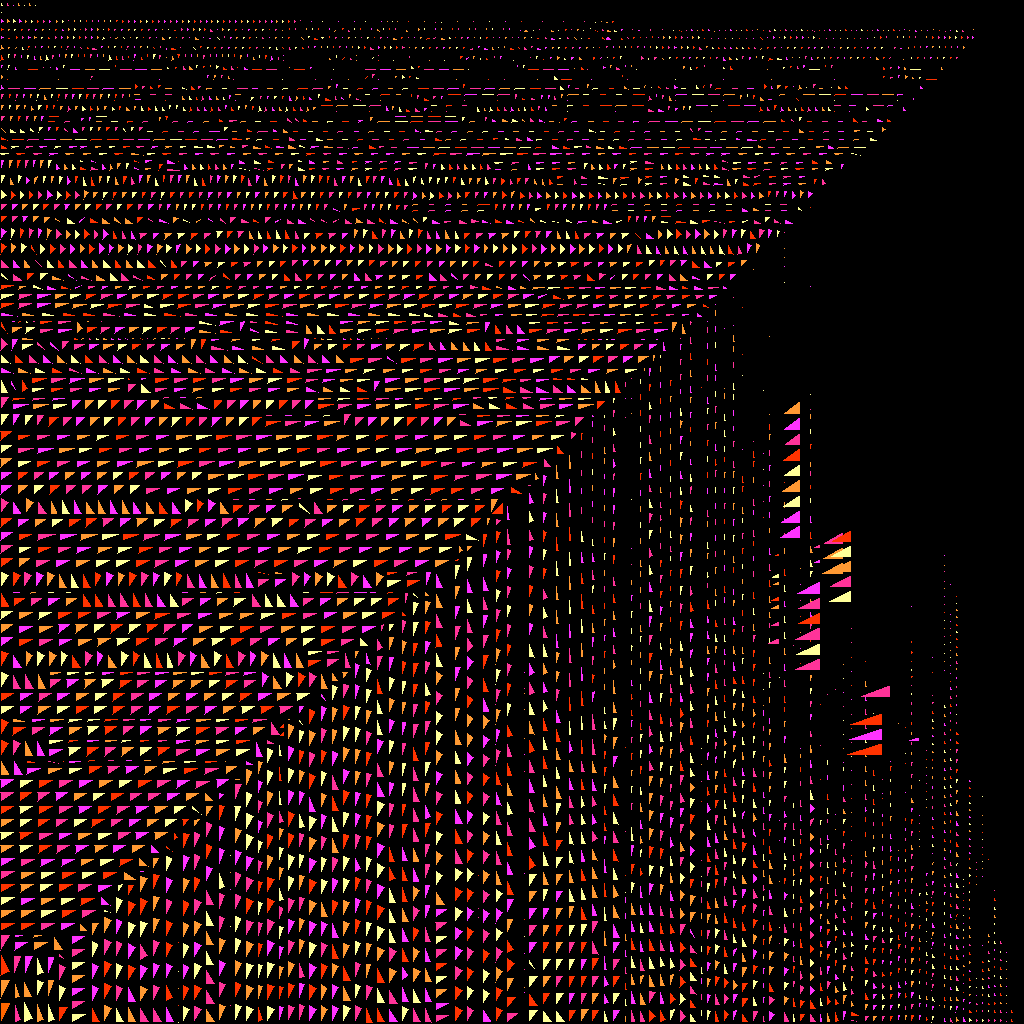
\includegraphics[scale=0.09]{images/previously_work/teapot/texel_dump.png}}\qquad
\subfigure[AO texture]{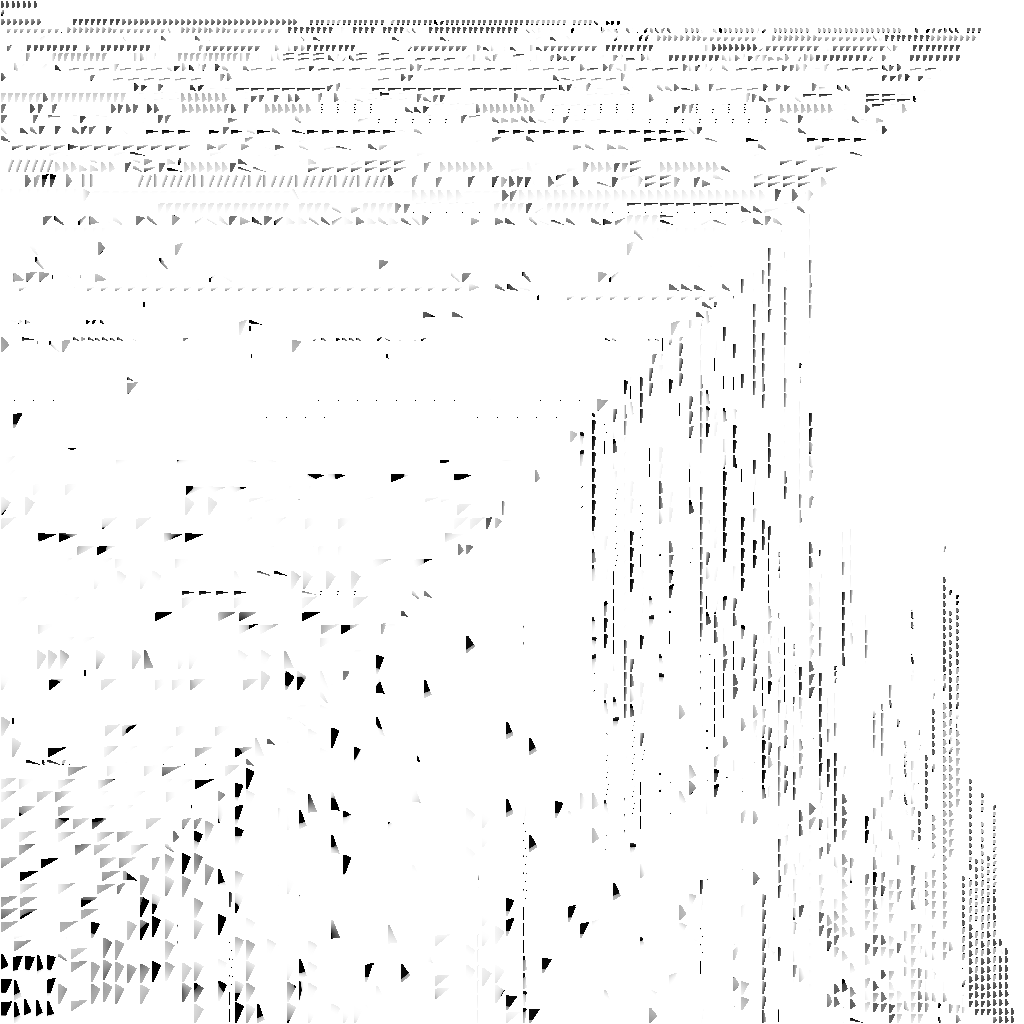
\includegraphics[scale=0.09]{images/previously_work/teapot/texture.png}}
\caption{output delle fasi intermedie per il modello teapot.obj}
\label{img:test_teapot}
\subfigure[packing del piano]{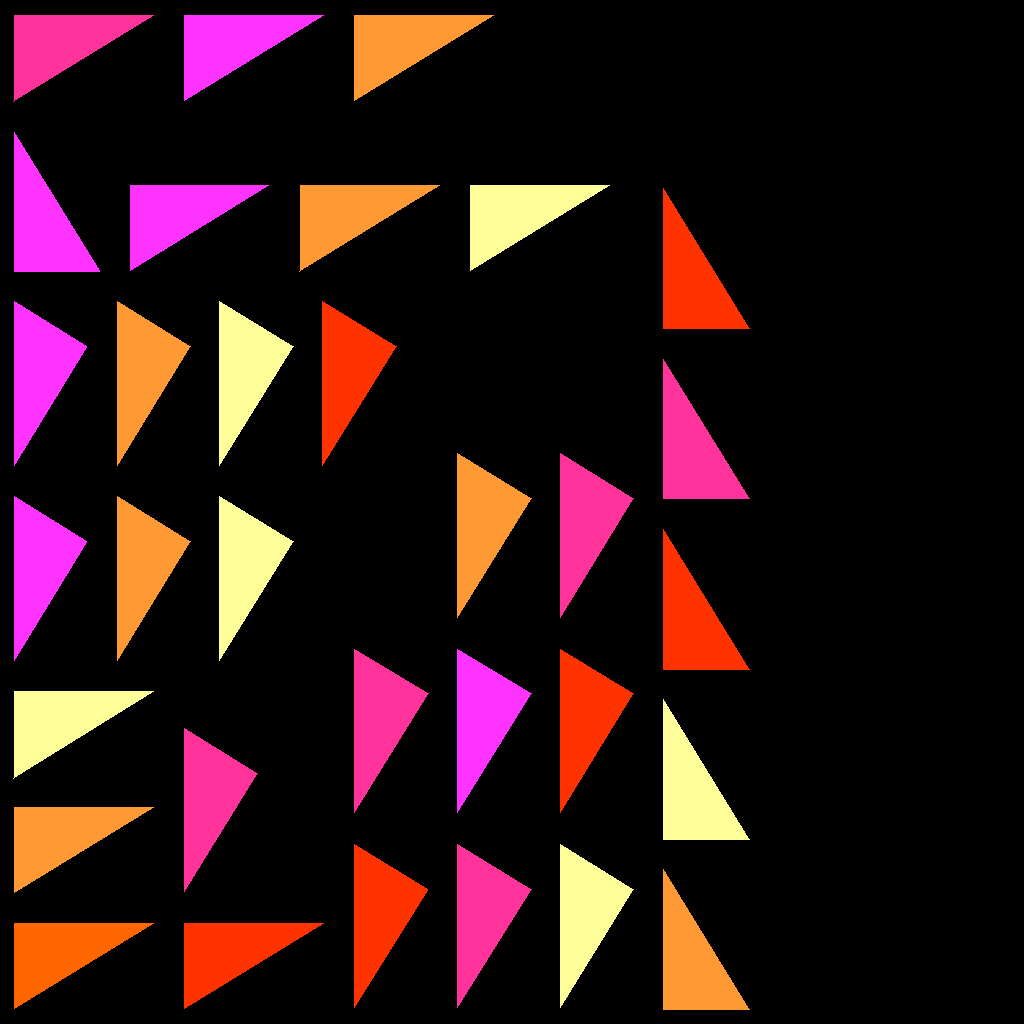
\includegraphics[scale=0.08]{images/previously_work/test/texel_dump_plan.png}}\qquad
\subfigure[packing della sfera]{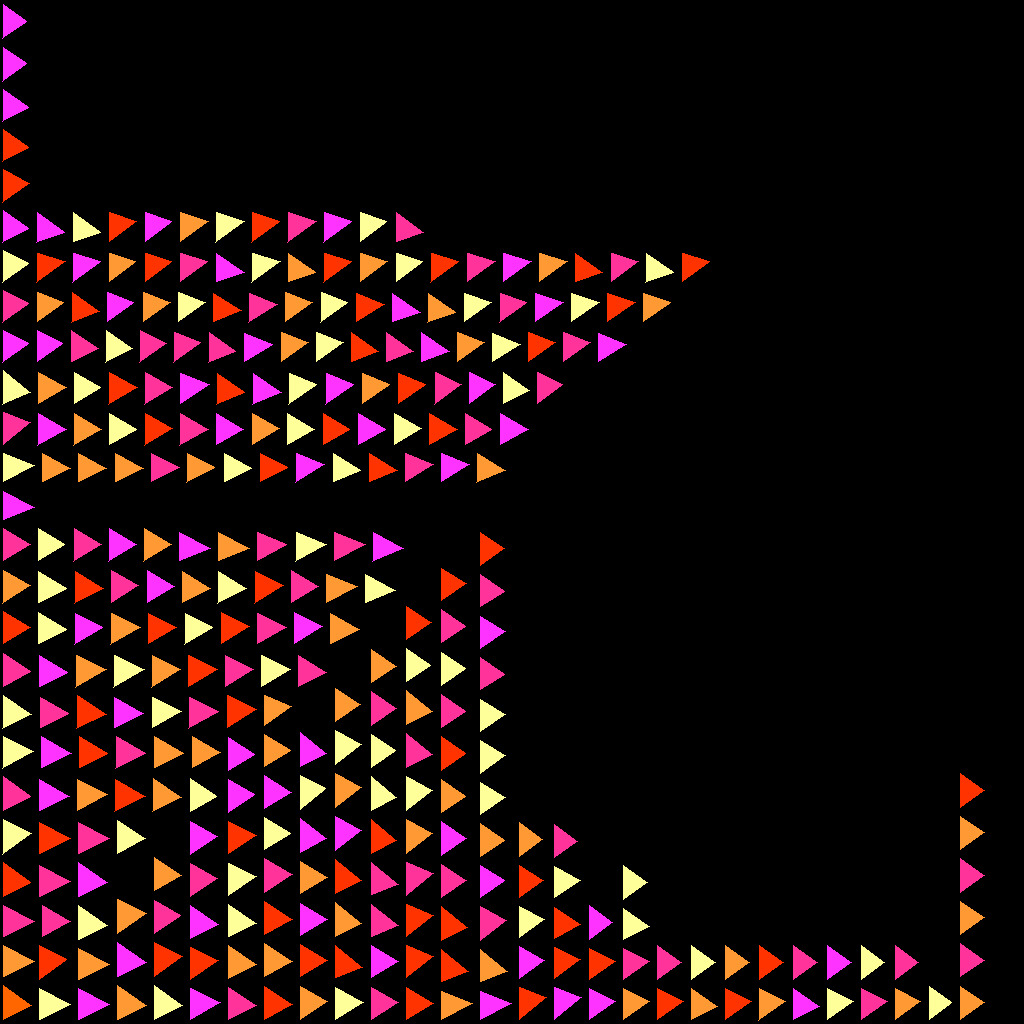
\includegraphics[scale=0.08]{images/previously_work/test/texel_dump_sphere.png}}\qquad
\subfigure[AO texture piano]{
\includegraphics[scale=0.08]{images/previously_work/test/texture_plan.png}}\qquad
\subfigure[AO texture sfera]{
\includegraphics[scale=0.08]{images/previously_work/test/texture_sphere.png}}
\caption{output delle fasi intermedie per il modello prova.obj}
\label{img:test_prova}
\end{figure}

Gli stessi problemi verificatesi con il modello monkey.obj si presentano anche questi modelli. Nell'immagine \ref{img:test_output} si pu� osservare come si presentano le scene in uscita con applicate le texture, mentre nell'immagine \ref{img:teapot_alter} e \ref{img:test_alter}  si vedono i dettagli delle alterazioni non desiderate.

\begin{figure}[!h]
\centering %
\subfigure[teapot.obj]{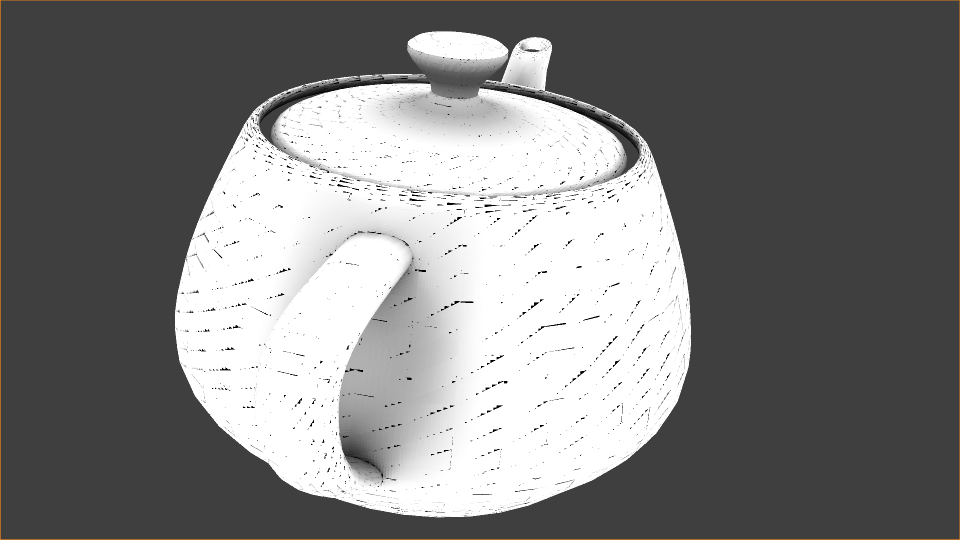
\includegraphics[scale=0.20]{images/previously_work/teapot/final_output.png}}\qquad
\subfigure[prova.obj]{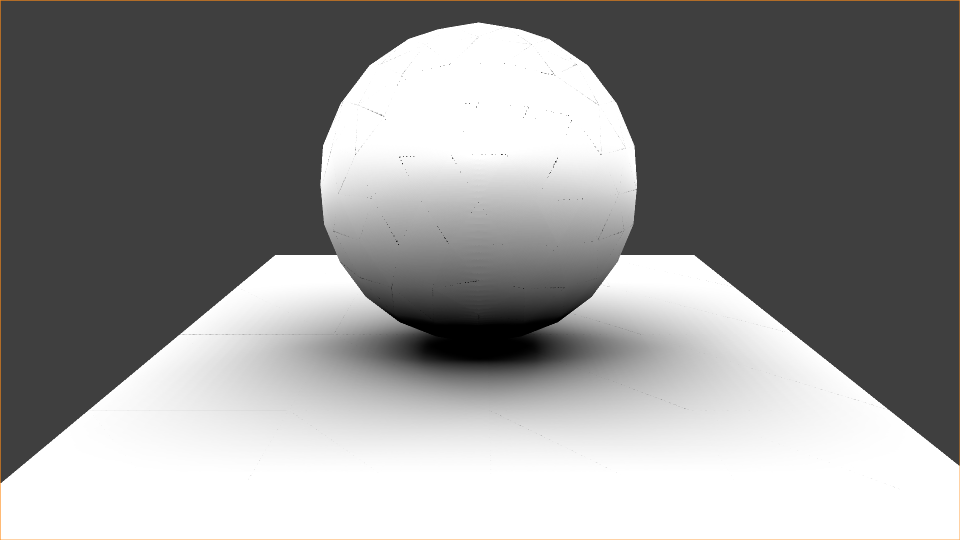
\includegraphics[scale=0.20]{images/previously_work/test/final_output.png}}
\caption{output finali}
\label{img:test_output}
\end{figure}

\begin{figure}[!h]
\centering %
\subfigure[tagli]{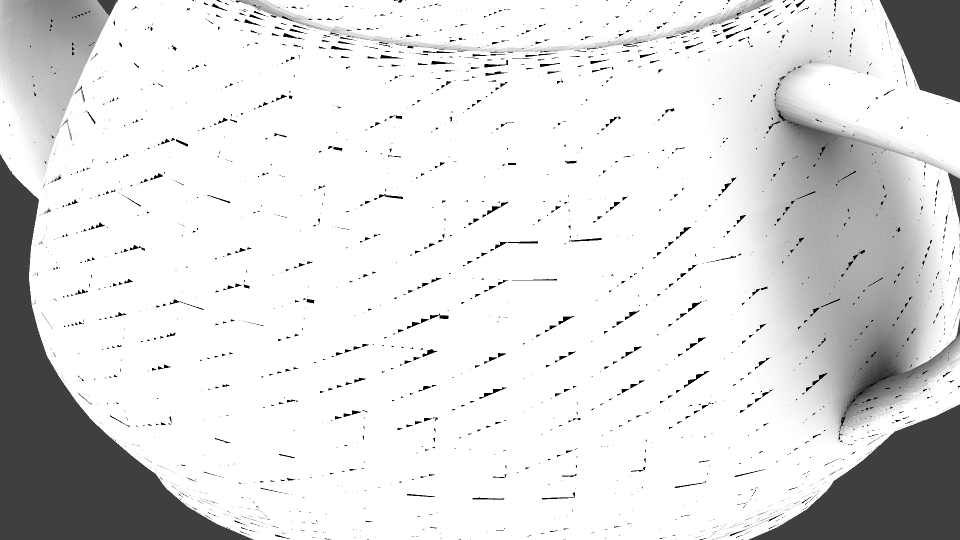
\includegraphics[scale=0.15]{images/previously_work/teapot/cuts.png} \label{img:teapot_prova_cuts}}\qquad\qquad
\subfigure[discontinuit�]{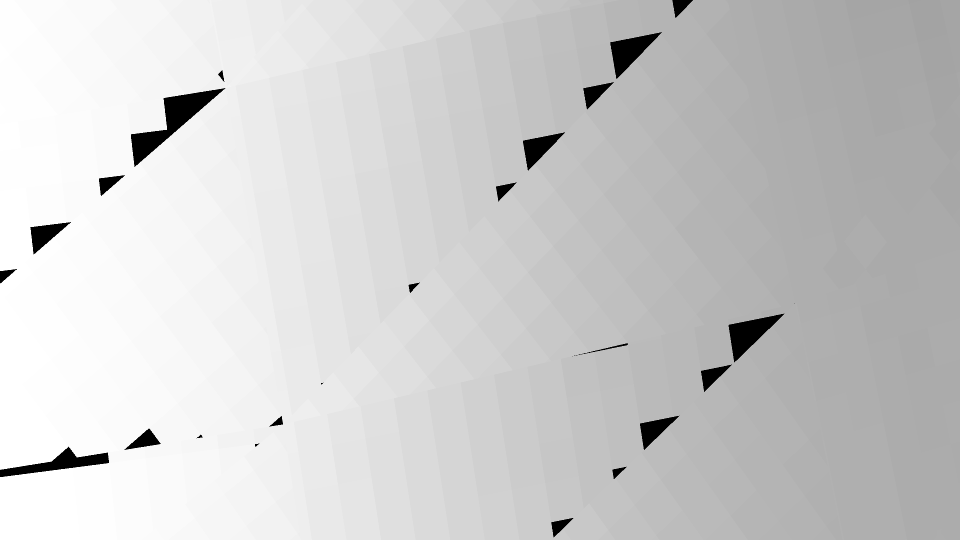
\includegraphics[scale=0.15]{images/previously_work/teapot/discontinuity.png} \label{img:teapot_prova_disc}}
\caption{dettagli relativi al modello teapot.obj}
\label{img:teapot_alter}
\end{figure}

\begin{figure}[!h]
\centering %
\subfigure[tagli]{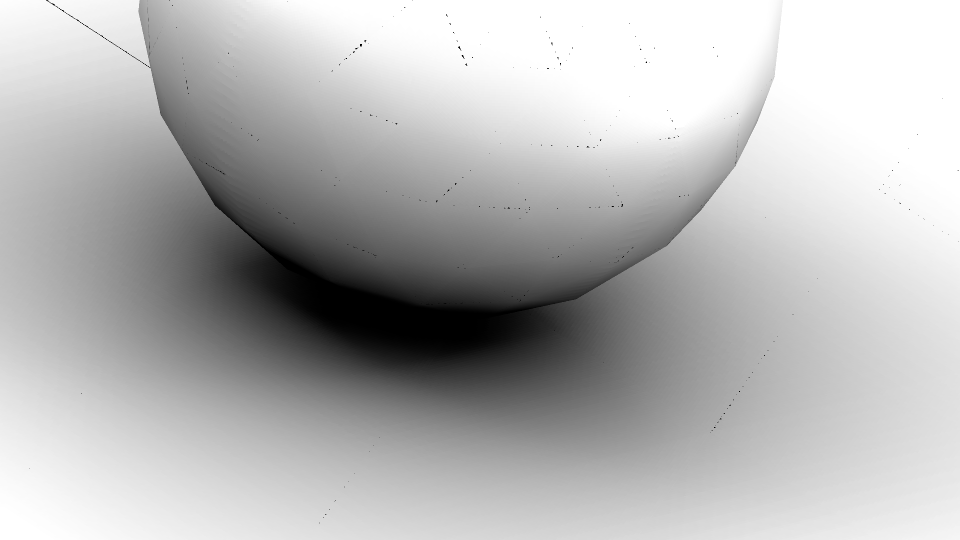
\includegraphics[scale=0.15]{images/previously_work/test/cuts.png} \label{img:test_prova_cuts}}\qquad\qquad
\subfigure[discontinuit�]{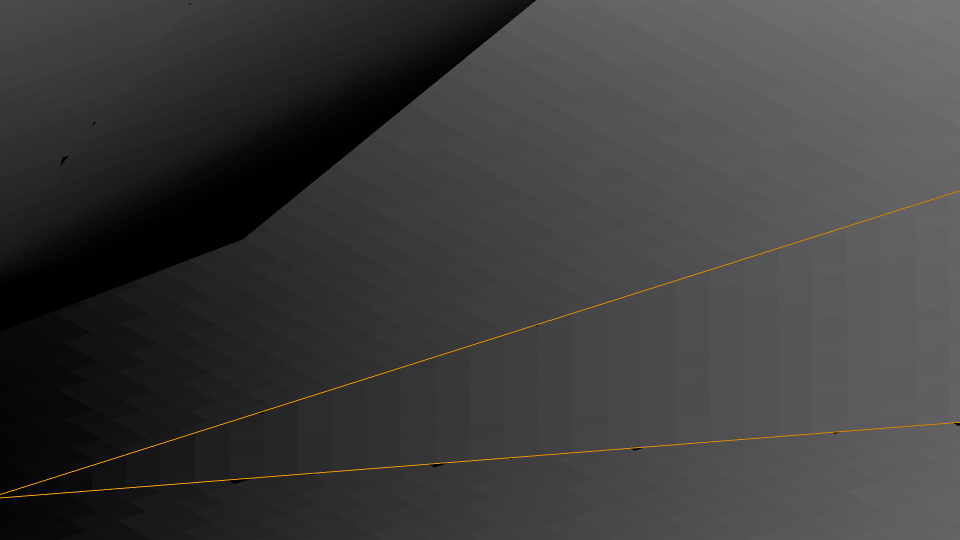
\includegraphics[scale=0.15]{images/previously_work/test/discontinuity.png} \label{img:test_prova_disc}}
\caption{dettagli relativi al modello prova.obj}
\label{img:test_alter}
\end{figure}

\subsection{Valutazioni finali}
Abbiamo potuto osservare che i risultati ottenuti non soddisfano i requisiti di resa grafica desiderata. Mentre non si osservano particolari problemi negli output intermedi del programma, sono almeno due le alterazioni non desiderate dovute all'applicazione della texture sulla superficie. L'alterazione pi� evidente � certamente quella visibile nelle immagini \ref{img:test_prova_cuts} e \ref{img:teapot_prova_cuts}, in cui si osservano delle striscie nere presenti sull'intera superficie. Questa � dovuta al fatto che per alcuni triangoli non vengono generati sufficienti texel per ricoprire l'intera superficie in $O_{uv}$.

La seconda problematica riscontrata � la discontinuit� presente tra i pixel di facce adiacenti (figura \ref{img:test_prova_disc} e \ref{img:teapot_prova_disc}). La ragione � da ricercarsi probabilmente nel fatto che facce adiacenti sulla mesh sono mappati con aree distanti tra loro. Considerando che le aree in Ouv vengono rasterizzate tutte nello stesso verso, una volta applicata la texture sulla mesh, non si pu� garantire che l'orientazione  dei pixel su facce differenti della mesh sia la stessa per facce adiacenti (per via delle disposizioni differenti delle aree in $O_{uv}$). %**si pu� migliorare [immagine che spiega il concetto]

La risoluzione della prima problematica richiede di rivedere l'algoritmo utilizzato per il calcolo dei texel, probabilmente non sar� necessario applicare grandi modifiche. Per eliminare le discontinuit� sar� necessario ripensare interamente l'algoritmo di unwrapping, infatti per risolvere questo problema � necessario che facce adiacenti sulla mesh siano mappate in aree anch'esse adiacenti. Nel prossimo capitolo discuteremo la risoluzione dettagliata dei problemi riscontrati con il programma iniziale.

\section{Progetto}

L'obiettivo � quello di revisionare il programma gi� esistente in modo da rispettare appieno le specifiche richieste. Vogliamo ottenere un programma che sia in grado di calcolare l'AO texture associata a una scena. La texture ottenuta deve essere il pi� possibile simile a quello che si otterrebb� calcolando direttamente l'AO in tempo reale sulla geometria. Questo programma renderebbe possibile precalcolare l'AO associato a grandi scene e salvarne il risultato, permettendo di risparmiare tempo durante la renderizzazione della scena.

\subsection{Analisi delle specifiche}
Descriviamo ora brevemente le specifiche che il programma deve rispettare. Le specifiche sono definite solamente sui dati in ingresso e sui risultatati attesi, non si richiedono particolarit� sul metodo seguito per ottenerli.

Il programma deve essere in grado di prendere in input da linea di comando il nome di un file (compreso di directory) contenente i dati sulla scena. Questo file sar� in un formato standard per la rappresentazione delle mesh, in particolare nei formati obj e osb (formato per OpenSG). Oltre a questo il programma non avr� a disposizione nessuna altra informazione sulla scena, eventuali dati necessari per il calcolo del risultato dovranno essere ricavati durante l'elaborazione.

In uscita si dovr� ottenere un file identico a quello preso in ingresso (stesso formato) con in pi� applicata la texture dell'AO. L'obiettivo � quello di calcolare l'AO dell'intera scena e aggregarla alla scena stessa come texture, il programma dovr� quindi eventualmente calcolare le coordinate UV e disporle sul piano della texture.

Eventualmente il programma dovr� fornire informazioni aggiuntive utili per il debug in caso di errore. Non si richiede un particolare formato o struttura per le eventuali informazioni di debug in uscita, queste dovranno solamente essere espresse in modo chiaro, conciso e riportare in maniera coerente con la struttura del programma. %(da rivedere) concetto blocco info 1 - > fase 1 del programma.

Il programma dovr� essere in grado di operare su qualsiasi mesh data in ingresso. Nel caso in cui non sia in grado di ottenere la scena in uscita, dovr� fornire sufficienti informazioni sulla tipologia di problema riscontrato in modo tale da permetterne il debug. %**non contrasta con quello che ho scritto sopra?

\subsection{Risoluzione problematiche riscontrate}
Nel capitolo precedente abbiamo gi� analizzato i risultati ottenuti fino ad ora. Le specifiche stilate vengono tutte soddisfatte dalla prima versione del programma eccetto
per alcune imperfezioni sull'applicazione della texture alla scena. Ci concentreremo quindi sulla risoluzione delle problematiche riscontrate analizzandole e discutendo
i possibili approcci da seguire per migliorare la resa della texture.

\subsubsection{Texel mancanti}
Il problema che pi� si nota � sicuramente quello dovuto all'applicazione della texture sulle singole facce che porta ad avere porzioni di mesh non ricoperte. Come gi� discusso
l'origine di queste alterazioni � da ricercarsi nella fase di calcolo dei texel, per qualche motivo l'algoritmo non riesce a ricavare texel sufficienti a ricoprire interamente
le facce della mesh.

%Descriviamo ora brevemente l'algoritmo utilizzato per il calcolo dei texel (pseudocodice x) e cerchiamo di proporre una versione differente dell'algoritmo stesso. TODO descrivere l'algoritmo [pseudocodice]
%TODO come risolverlo -> contorni

\subsubsection{Discontinuit�}
La seconda problematica riscontrata � la discontinuit� della texture presente sulle facce adiacenti della mesh. Abbiamo effettuato alcuni test e abbiamo notato che questo problema si presenta  maggiormente con texture di piccole dimensioni. Nell'immagine \ref{img:prev_work} mettiamo a confronto l'applicazione di texture di differenti dimensioni sul modello prova.obj (le texture sono state calcolate con la prima versione del programma). Il motivo per cui le discontinuit� sono pi� visibili con texture di piccole dimensioni � che la dimensione del pixel sulla faccia della mesh � inversamente proporzionale alla dimensione della texture.

\begin{figure}[!h]
\centering %
\subfigure[256px x 256px senza filtro]{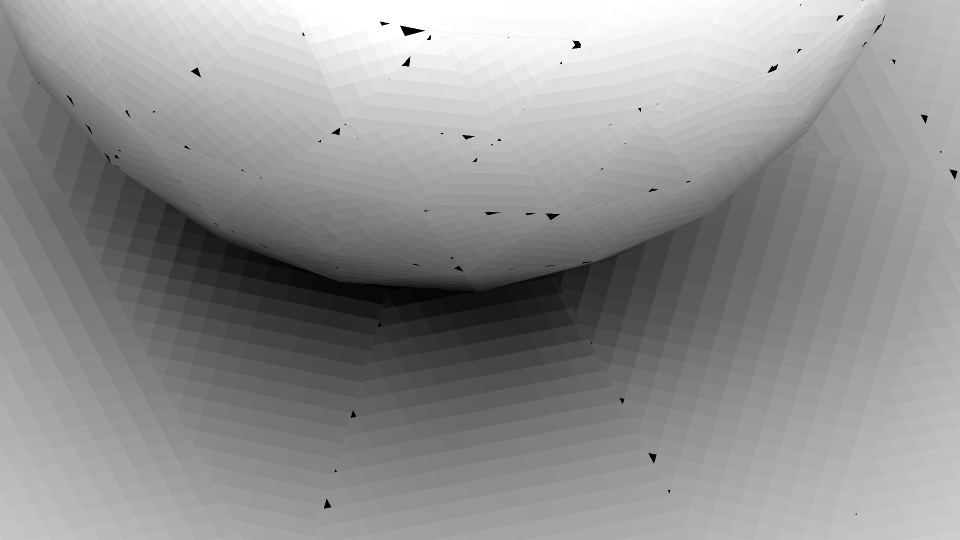
\includegraphics[scale=0.13]{images/previously_work/discontinuity/prova_256.png}}\qquad 
\subfigure[512px x 512px senza filtro]{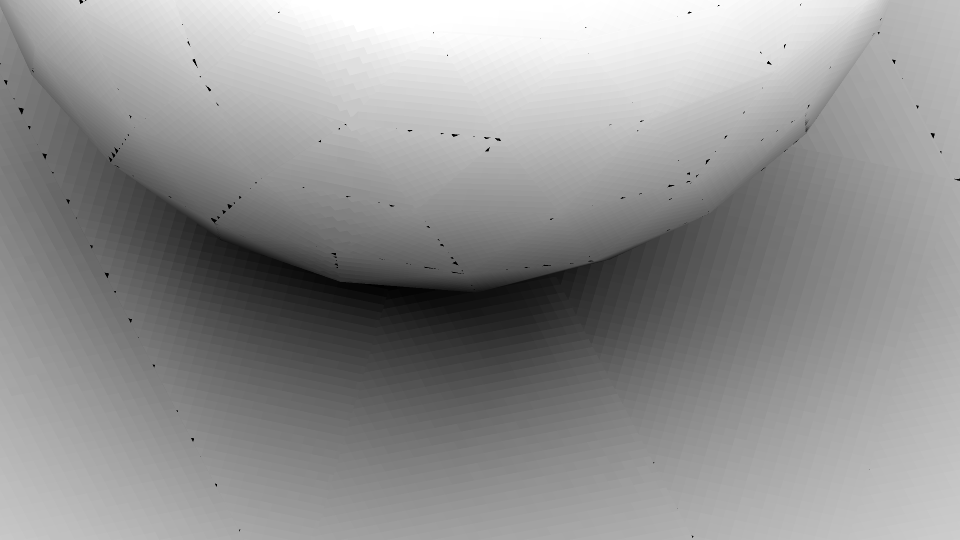
\includegraphics[scale=0.13]{images/previously_work/discontinuity/prova_512.png}}\qquad 
\subfigure[1024px x 1024px senza filtro]{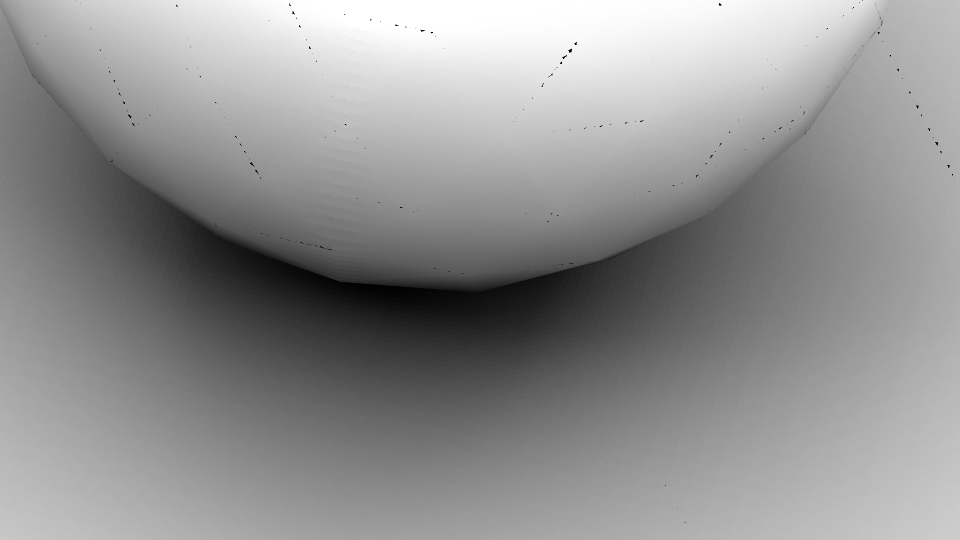
\includegraphics[scale=0.13]{images/previously_work/discontinuity/prova_1024.png}}\qquad 
\label{img:prev_work}
\end{figure}

Il problema � dovuto ai diversi versi di rasterizzazione seguiti da superfici adiacenti sulla mesh. Per risolvere il problema si possono seguire diversi approcci che operano a livelli differenti del programma. Una possibile soluzione prevede che la scena in output venga renderizzata applicando alla texture un particolare filtro, seguendo le false righe di quello che fa' Blender. Nell' immagine \ref{img:prev_work_filter} possiamo vedere come aumenta la resa delle texture applicando l'opzione Mipmaps di Blender (File \textrightarrow User Preferences \textrightarrow System \textrightarrow OpenGL). 

\begin{figure}[!h]
\centering %
\subfigure[256px x 256px senza filtro]{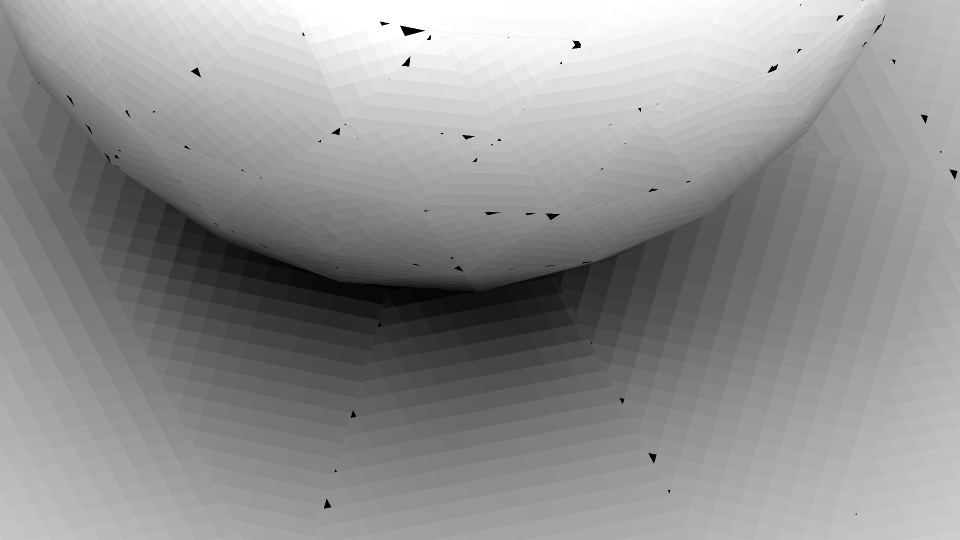
\includegraphics[scale=0.12]{images/previously_work/discontinuity/prova_256.png}}\qquad 
\subfigure[512px x 512px senza filtro]{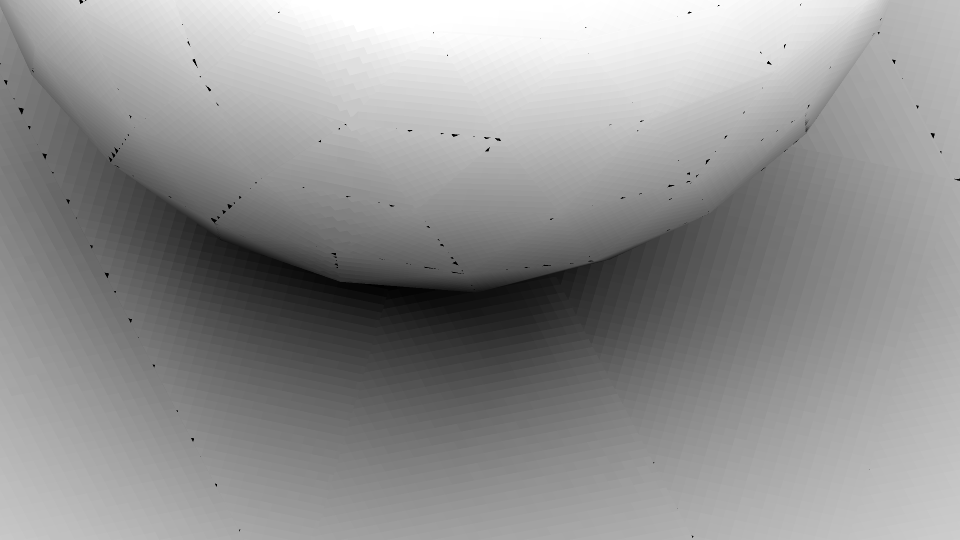
\includegraphics[scale=0.12]{images/previously_work/discontinuity/prova_512.png}}\qquad 
\subfigure[1024px x 1024px senza filtro]{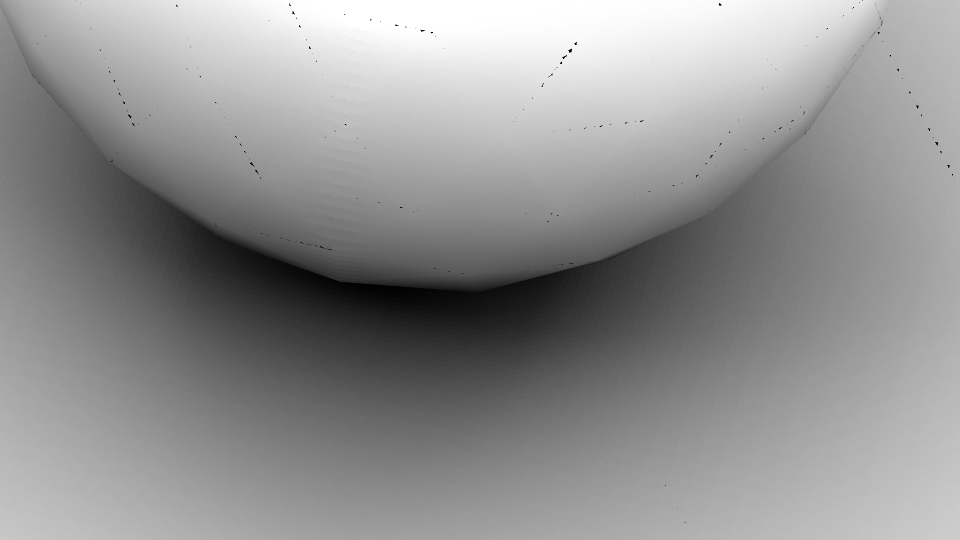
\includegraphics[scale=0.12]{images/previously_work/discontinuity/prova_1024.png}}\qquad 
\subfigure[256px x 256px con filtro]{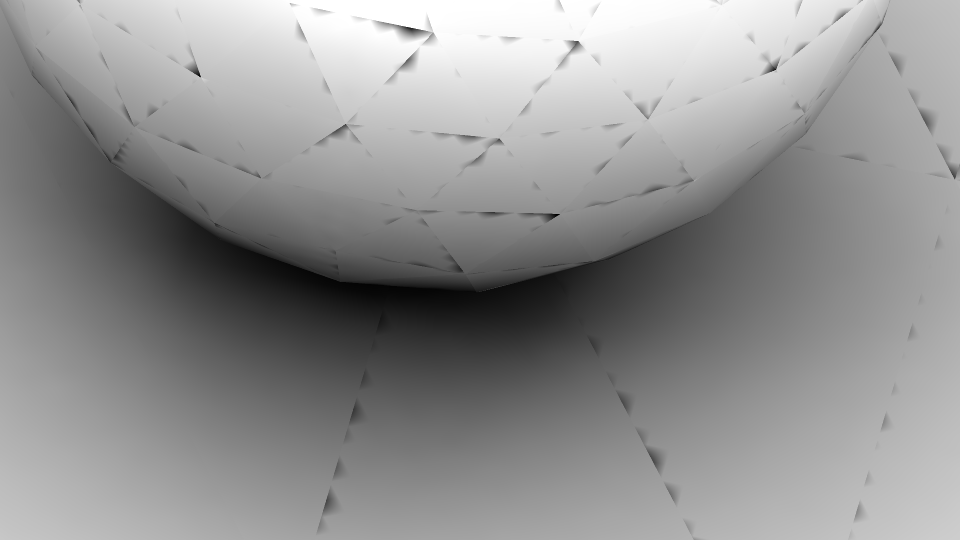
\includegraphics[scale=0.12]{images/previously_work/discontinuity/prova_256_filtrata.png}}\qquad 
\subfigure[512px x 512px con filtro]{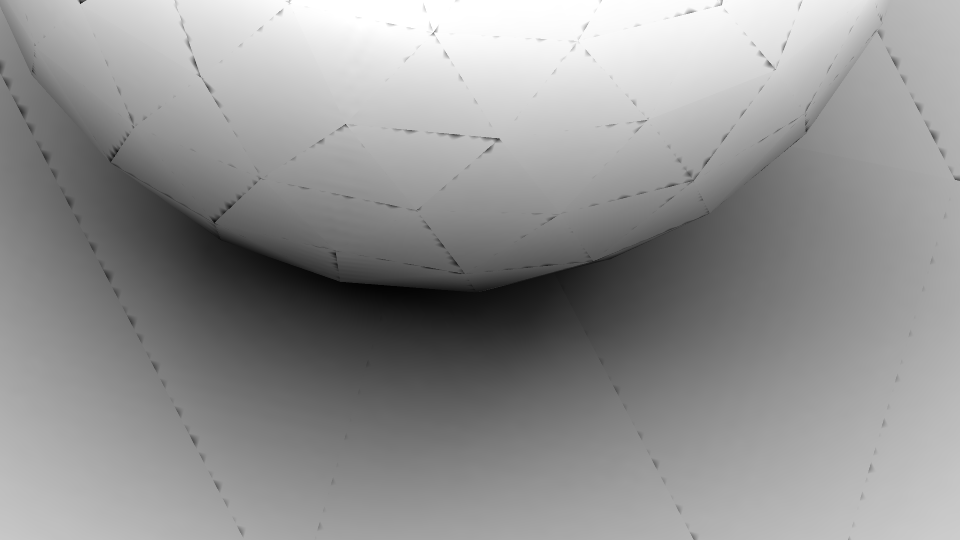
\includegraphics[scale=0.12]{images/previously_work/discontinuity/prova_512_filtrata.png}}\qquad 
\subfigure[1024px x 1024px con filtro]{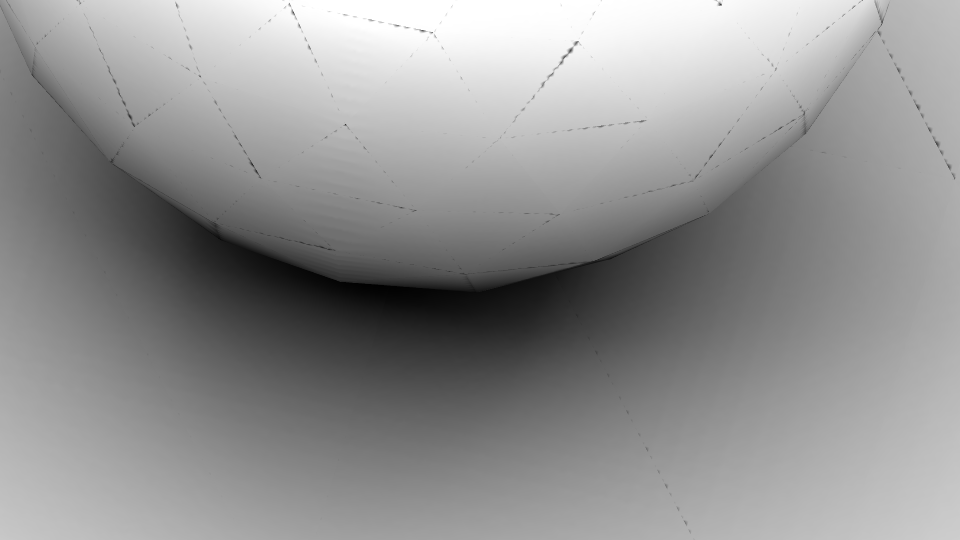
\includegraphics[scale=0.12]{images/previously_work/discontinuity/prova_1024_filtrata.png}}\qquad  
\caption{confronto delle texture con e senza filtro}
\label{img:prev_work_filter}
\end{figure}

Si pu� notare una netta diminuizione delle discontinuit� dovuta all'applicazione del filtro. Per quanto riguarda il problema dovuto alla non presenza dei texel questo non viene migliorato,
anzi si pu� osservare un aumento della visibilit� del fenomeno. Inoltre questo metodo � dipendente dall'applicativo utilizzato per aprire la scena, se questo non implementasse (oppure non attivasse)
la funzionalit� di filtro della texture allora non si otterrebbe nessun miglioramento. Per questo motivo considereremo questo approccio non utilizzabile.

In alternativa � possibile seguire un approccio che si basa sulla disposizione delle aree in $O_{uv}$. Il principio di base � che per prevenire le discontinuit� sia necessario disporre i triangoli adiacenti
nella mesh in modo adiacente nel piano $O_{uv}$. Bisogna quindi utilizzare un algoritmo di unwrapping che sia in grado di mantenere l'adiacenza tra la maggior parte dei vertici della mesh.
Procederemo quindi a una completa revisione dell'algoritmo di unwrapping utilizzato nell'applicativo.
Per il calcolo dell'unwrapping utilizzeremo un metodo che utilizza i principi della programmazione matematica
per minimizzare il discostamento in termini di angoli tra la mesh e l'area in $O_{uv}$. Utilizzeremo una versione modificata dell'algoritmo ABF++ \cite{cit:abf}, frutto del lavoro di Sheffer A. e De Sturler pubblicato nel 2001.
Nella sezione \ref{sec:aabf} tratteremo in dettaglio il funzionamento dell'algoritmo e le modifiche apportategli per rispondere alle nostre necessit�.

\subsection{Struttura del programma}
La struttura originale del programma rimarr� pressoch� inalterata, verranno invece aggiunte nuove funzionalit�. Il programma manterr� la strutturazione in fasi della prima versione (sezione \ref{subsez:program_struct}), il listato \ref{alg:prog_struct} ne riassume i principali passi.

\begin{algorithm}[!htb]
\caption{Algoritmo di ricostruzione}
\label{alg:prog_struct}
\begin{algorithmic}[1]
\Procedure{ParametrizzazioneScena} {Scena S}
	\State Vector[Geometria] geometrie = S.estraiGeometrie();
	\State Vector[Texel] texels;
	\For{Geometria G = geometrie.inizio(); G != geometrie.fine(); G = geometrie.estraiProssimaGometria(G)}
		\State G.convertiInNoIndici();
		\State
		\State OttieniParametrizzazioneUV(G);
		\State DisponiSuperfici(G);
		\State 
		\State texels = calcolaTexels(G);
		\State Immagine texture = calcolaAO(G, texels);
		\State ApplicaTexture(G, texture);
		\State
		\State LiberaMemoria(texels, texture);
	\EndFor
\EndProcedure
\end{algorithmic}
\end{algorithm}

Le principali modifiche riguarderanno la struttura dati, l'algoritmo di unwrapping e l'algoritmo di costruzione dei texel. Procederemo ora con la trattazione delle principali modifiche nello stesso
ordine in cui sono state affrontate durante l'implementazione.


\chapter{Algoritmi}

\section{Automatic-ABF} \label{sec:aabf}

\subsection{Introduzione}
La parametrizzazione definisce una corrispondenza tra la mesh 3D e un dominio 2D chiamato spazio di parametrizzazione. L'associazione generata dalla parametrizzazione dovrebbe
assicurare una corrispondenza biunivoca tra i due insiemi. Nelle applicazioni pratiche garantire la corrispondenza biunivoca locale � sufficiente, questo si ottiene se nello
spazio di parametrizzazione non sono presenti triangoli sovvrapposti.

I principali usi della parametrizzazione sono il texture mapping e il geometry editing. Per queste applicazioni la qualit� del risultato dipende fortemente dall'ammontare
delle deformazioni causate dalla parametrizzazione. Idealmente, durante la mappatura, si dovrebbero presevare le aree e gli angoli di tutte le facce ottenendo cos� una
trasformazione isometrica tra i due spazi. Solamente la classe delle superfici sviluppabili ammette una parametrizzazione isometrica, quindi nella pratica sono usati metodi
di parametrizzazione che si basano sulla minimizzazione della distorsione della parametrizzazione.

\subsection{ABF}
Il metodo ABF (angle based flatteling) si basa sull'osservazione che l'insieme degli angoli di una superficie 2D triangolarizzata la definisce univocamente (ad eccezione di
possibili scalamenti e trasformazioni rigide). La procedura utilizzata dall'ABF per prima cosa determina la parametrizzazione nello spazio degli angoli, successivamente
ricava le coordinate 2D. La formulazione del metodo lo porta ad essere particolarmente adatto per ridurre la distorsione angolare della mappatura.
%definzione taglio e vertici interni.

\subsubsection{Formulazione}
Il metodo ABF si basa sulla formulazione del problema attraverso un modello di programmazione non lineare. Definisce quindi una funzione obiettivo da minimizzare, insieme
ad una serie di vincoli che la soluzione deve rispettare. Nello spazio degli angoli la funzione obiettivo da minimizzare � semplicemente 
\begin{eqnarray}   E(\alpha) = \sum_{t \in T} { \sum_{k=1}^{3} {\frac{1}{w_k^t}{(\alpha_k^t - \beta_k^t)}^2 }} \end{eqnarray} 
dove $\alpha_k^t$ sono gli angoli planari (le nostre incognite) e $\beta_k^t$ sono gli angoli ottimali (angoli della mesh 3D). L'indice $t$ varia nell'insieme $T$ dei triangoli della mesh, mentre
l'indice $k$ varia sugli angoli di ciascun triangolo. I pesi $w_k^t$ sono impostati al valore $\frac{1}{{b_k^t}^2}$ per riflettere la distorsione relativa, piuttosto che utilizzare la distorsione
assoluta.

L'impostazione del problema di minimizzazione garantisce la biettivit� locale della parametrizzazione grazie ai vincoli imposti. Durante la risoluzione gli angoli vengono scalati
pi� volte per garantire una soluzione che definisca una parametrizzazione planare valida. Lo spazio delle soluzione viene quindi ridotto spazialmente dai seguenti vincoli
sulle variabili
\begin{itemize}
\item 
Validit� triangolare: ogni triangolo della mesh deve rimanere tale durante la parametrizzazione.
$$V_{Tri}(t) = \alpha_1^t + \alpha_2^t + \alpha_3^t=0, \; \forall t \in T$$
\item Planarit�: ogni vertice della mesh interno alla parametrizzazione deve verificare il vincolo di planarit�.
 $$V_{Plan}(v) = \sum_{(t,k) \in v^*} {\alpha_k^t -2\uppi}=0, \; \forall v \in V_{Int} $$
Dove $V_{Int}$ � l'insieme dei vertici interni alla superficie 2D e $v^*$ � il set degli angoli incidenti al vertice $v$.
\item Integrit� delle raggiere: ogni edge condiviso tra due triangoli deve avere la stessa lunghezza.
$$V_{Len}(v) = \prod_{(t,k) \in v^*} {\sin {\alpha_{k+1}^t}} - \prod_{(t,k) \in v^*} {\sin {\alpha_{k-1}^t}}, \; \forall v \in V_{Int}$$
Gli indici $k+1$ e $k-1$, indicano rispettivamente il prossimo e il precedente angolo del triangolo.
\end{itemize}

% \subsubsection{Vincolo di integrit� delle raggiere}

Analizziamo in dettaglio il vincolo di integrit� delle raggiere. Per prima cosa definiamo la raggiera di centro $v$ come l'insieme dei triangoli aventi $v$ come vertice in comune. Il vincolo garantisce che ogni edge condiviso tra due triangoli della raggiera abbia la stessa lunghezza, in caso contrario potrebbe verificarsi una situazione come quella in figura \ref{fig:alg_aabf_whell}. 

\begin{figure}[!htb]
\centering %
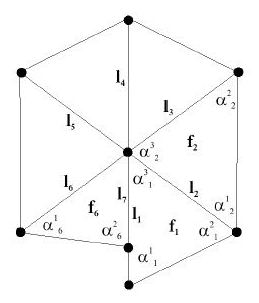
\includegraphics[scale=0.7]{images/algorithms/aabf/whell.jpg}
\caption{raggiera}
\label{fig:alg_aabf_whell}
\end{figure}

Questo vincolo viene espresso in funzione degli angoli esterni della raggiera. Partendo da una coppia di triangoli dobbiamo garantire che l'edge in comune abbia la stessa lunghezza, ci� si pu� esprime come
\begin{eqnarray}  
\frac{l_1}{l_2} = \frac{\sin{\alpha_1^2}}{\sin{\alpha_1^1}}
\end{eqnarray}
procedendo in maniera iterativa lungo la raggiera e in senso antiorario si ottiene
\begin{eqnarray}   
\frac{l_2}{l_3} & = & \frac{\sin{\alpha_2^2}}{\sin{\alpha_2^1}} \\  
\frac{l_1}{l_3} & = & \frac{l_1 l_2}{l_2 l_3} = \frac{\sin{\alpha_1^2}}{\sin{\alpha_1^1}} \cdot \frac{\sin{\alpha_2^2}}{\sin{\alpha_2^1}} \\
\frac{l_1}{l_7} & = & \frac{l_1}{l_2} \cdot \frac{l_2}{l_3} \cdot\cdot\cdot \frac{l_6}{l_7} = \frac{\sin{\alpha_1^2}}{\sin{\alpha_1^1}} \cdot\cdot\cdot \frac{\sin{\alpha_2^2}}{\sin{\alpha_2^1}}  \frac{\sin{\alpha_6^2}}{\sin{\alpha_6^1}}
\end{eqnarray}
Considerando che abbiamo bisogno che $l_7 = l_1$ per ricostruire la raggiera, si ottiene
\begin{eqnarray}   
\frac{\sin{\alpha_1^2}}{\sin{\alpha_1^1}} \cdot\cdot\cdot \frac{\sin{\alpha_2^2}}{\sin{\alpha_2^1}}  \frac{\sin{\alpha_6^2}}{\sin{\alpha_6^1}} = 1
\end{eqnarray}
Una volta fissata la raggiera (e il vertice centrale $v$), il vincolo pu� essere espresso come la differenza di due produttorie. La prima contiene il prodotto dei seni degli angoli destri esterni della raggiera, mentre la seconda il prodotto dei seni degli angoli sinistri esterni della raggiera, in formule
\begin{eqnarray}   
\prod_{\alpha \in A_{estDx}} {\sin {\alpha}} - \prod_{\alpha \in A_{estSx}} {\sin {\alpha}} = 0
\end{eqnarray}
dove $A_{estDx}$ � l'insieme degli angoli esterni destri della raggiera, mentre $A_{estSx}$ � l'insieme degli angoli esterni sinistri della raggiera.

\subsubsection{Meccanismo di risoluzione}
Per la risoluzione del problema abbiamo utilizzato una libreria esterna IpOpt \cite{cit:ipopt}. La libreria implementa una serie di algoritmi per la determinazione di problemi di programmazione non lineare. IpOpt � scritto interamente in C++ e permette di interfacciarsi con altri programma attraverso l'uso e l'estensione di classi. In particolare richiede che il programma client estenda la classe {\scshape TNLP} e che richieda la risoluzione attraverso la classe {\scshape IpoptApplication} caricata da una libreria dinamica esterna.

La classe {\scshape ZedABFProblem} del programma estende le funzionalit� della classe {\scshape TNLP} di IpOpt. Nell'implementazione sono presenti vari metodi richiesti da IpOpt, tra i principali: 
\begin{itemize}
\item 
{\scshape get\_nlp\_info}: questo metodo ritorna alcune informazioni sulla dimensione del problema non lineare, utili alla libreria per allocare sufficiente area di memoria per l'esecuzione;
\item 
{\scshape get\_bounds\_info}: questo metodo definisce per ciascuna variabile il dominio di appartenenza;
\item 
{\scshape get\_starting\_point}: questo metodo assegna un punto di partenza per il problema NLP, viene usato nel caso in cui si utilizzi un'euristica che restituisca una soluzione vicini all'ottimo;
\item 
{\scshape eval\_f}: restituisce il valore della funzione obiettivo nel punto assegnato;
\item 
{\scshape eval\_grad\_f}: restituisce il valore del gradiente della funzione obiettivo nel punto assegnato;
\item 
{\scshape eval\_g}: calcola i valori dei vincoli nel punto assegnato;
\item 
{\scshape eval\_jac\_g}: pu� restituire la struttura della matrice Jacobiana associata ai vincoli, oppure il valore della matrice in un punto dato;
\item 
{\scshape eval\_h}: pu� restituire la struttura della matrice Hessiana della funzione obiettivo, oppure il valore della matrice in un punto dato;
\item 
{\scshape finalize\_solution}: questo metodo � chiamato quando l'algoritmo di ricerca dell'ottimo termina.
\end{itemize}

IpOpt richiede per la risoluzione del problema che sia implementata almeno il metodo {\scshape eval\_grad\_f} che restituisce il valore del gradiente $\bigtriangledown E(\alpha)$. Anche se non strettamente necessario, abbiamo implementato anche il metodo {\scshape eval\_jac\_g} che calcolo il valore della matrice Jacobiana associata ai vincoli del problema, questo permette di velocizzare il processo di risoluzione. In aggiunta era possibile implementare anche il metodo {\scshape eval\_h} per il calcolo della matrice Hessiana della funzione obiettivo.

% Nell'appendice A sono disponbili i codici sorgenti delle funzioni, mentre nell'appendice B sono presenti gli sviluppi matematici per il calcolo del gradiente di $E(\alpha)$ e della matrice Jacobiana, insieme ad altre considerazioni utili.

\subsubsection{Ricostruzione parametrizzazione}
Una volta determinata una soluzione per il problema di minimizzazione � necessario ricostruire la parametrizzazione a partire dagli angoli dello spazio 2D. L'algoritmo di ricostruzione si basa su di un metodo ricorsivo di ricostruzione delle singole raggiere. Per prima cosa fissa un triangolo iniziale da cui partire e successivamente si considera un suo vertice che verr� preso come seme. A partire dal vertice seme si procede con la ricostruzione della raggiera corrispondente, che prevede il calcolo della parametrizzazione di ogni singolo triangolo e la ricorsione su tutti i vertici esterni. Nel listato \ref{alg:abf_reconstruction} � descritto l'algortimo di ricostruzione.

\begin{algorithm}[!htb]
\caption{Algoritmo di ricostruzione}
\label{alg:abf_reconstruction}
\begin{algorithmic}[1]
\Procedure{Parametrizzazione2D} {Geometria G}
	\Require I triangoli di ogni raggiera di G devono essere ordinati in senso anti-orario.
	\State Triangolo t = G.estraiTriangolo(0); 
	\State Vertex seme = e.estraiVertice(0);
	\State Vertex b = e.estraiVertice(1);
	\State seme.inserisciPosizione2D(0, 0);
	\State a.inserisciPosizione2D(0, e.lunghezza());
	\State CostruzioneRaggiera2D(seme);
\EndProcedure
\Statex
\Procedure{CostruzioneRaggiera2D} {Vertice v, Triangolo t, Edge e}
	\State Raggiera R = v.estraiRaggiera();
	\While {t.estraiFlagParametrizzazione() == 0};
		\State ParametrizzaTriangolo(v, t, e);
		\State /* Parametrizza il triangolo t e imposta il suo flag di parametrizzazione a 1 */
		\State 
		\State (t,e) = R.etraiProssimoTriangolo(v, t, e);
		\State /* Estrai il triangolo adiacente a t e l'edge in comune e */
	\EndWhile
	\State
	\For{Vertex i = R.inizioVerticiEsterni(); i != R.fineVerticiEsterni(); i = R.estraiProssimoVertice(i)}
		\State Raggiera nuova\_r = i.estraiRaggiera();
		\State Triangolo prossimo\_t = nuova\_r.estraiPrimoTriangoloLibero();
		\State /* Estrae il primo in senso anti-orario triangolo non marcato con il flag di parametrizzazione. */
		\If{prossimo\_t != NULL}
			\State Triangolo precedente\_t = nuova\_r.estraiTriangoloPrecedente(prossimo\_t);
			\State /* Estrae il triangolo a destra di prossimo\_t all'interno di nuova\_r*/
			\State Edge prossimo\_e = precedente\_t.estraiEdgeComune(prossimo\_t);
			\State CostruzioneRaggiera2D(i, prossimo\_t, prossimo\_e);
		\EndIf
	\EndFor
\EndProcedure
\end{algorithmic}
\end{algorithm}

\subsection{Variazioni sull'ABF}
L'ABF richiede che si definisca l'insieme dei vertici interni nella parametrizzazione, o in modo equivalente l'insieme dei vertici esterni. I vertici esterni definiscono sulla mesh 3D il taglio lungo il quale si effettuer� l'unwrapping della superficie 3D. Per rispettare le specifiche richieste il taglio della mesh non potr� essere definito dall'utente, per questo motivo � necessario definire un metodo di creazione del taglio automatizzato.

Per garantire la capacit� del programma di parametrizzare sempre la mesh utilizzeremo un approccio per la creazione di pi� tagli. Per la determinazione di questi tagli sulla geometria procederemo con un approccio basato sulla visibilit� della geometria da diversi 'punti di vista'. Una volta determinati i tagli otterremmo una serie di sotto-mesh da parametrizzare, per ciascuna di esse utilizzeremo l'ABF per il calcolo della parametrizzazione. Ogni mesh generer� quindi un insieme di sotto-parametrizzazione che andrann� disposte sul piano Ouv della texture.

Descriveremo ora brevemente l'algoritmo per il calcolo dei tagli sulla mesh. Dato un vettore $v$ rappresentante la direzione di visione determiniamo tutti i triangoli che presentano una normale orientata in direzione opposta a $v$. Otterremmo quindi un sotto-superficie della mesh originale, da questa determineremo l'insieme delle superfici completamente collegate da raggiere. A questo punto per ogni sotto-superficie collegata si definisce l'insieme dei vertici esterni, cio� quei vertici tali per cui la raggiera associata non si chiude su se stessa oppure per cui la somma degli angoli interni � maggiore di $2\uppi$. Infine viene determinata la parametrizzazione per ciascuna sotto-superficie collegata, attraverso l'utilizzo del metodo ABF. Il listato \ref{alg:mesh_cut} mostra lo pseudocodice dell'algortimo utilizzato.

\begin{algorithm}[!h]
\caption{Algoritmo di parametrizzazione}
\label{alg:mesh_cut}
\begin{algorithmic}
\Procedure{ParametrizzaGeometria} {Geometria G}
	\State Vector[Vettore] direzioni = calcolaDirezioniOttimali(G);
	\For {Vettore v = direzioni.inizio(); v != direzioni.fine(); v = direzioni.prossimo(v)}
		\State Vector[Triangolo] triangoli = ottieniTriangoliVisibili(G, v);
		\State Vector[Superficie] s\_collegate = calcolaSuperficiColllegate(G, triangoli);
		\For{Superficie s = s\_collgate.inizio(); s != s\_collgate.fine(); s = s\_collgate.prossima(s)}
			\State Vector[Vertice] vertici\_esterni = s.ottieniVerticiEsterni();
			\State G.CollegaSuperficie(S);
			\If{vertici\_esterni.dimensione() != 0}
				\State CalcolaParametrizzazioneABF(G);
			\Else
				\State ImpostaSoluzioneIniziale3D(G);
				\State Parametrizzazione2D(G);
			\EndIf
			\State G.ScollegaSuperficie(S);
		\EndFor
	\EndFor
\EndProcedure
\end{algorithmic}
\end{algorithm}

\section{Greedy packing}

\subsection{Introduzione}
Una volta determinata le parametrizzazione della varie sotto-superfici � necessario disporre le aree ottenute nello spazio $O_{uv}$. L'obiettivo � quello di determinare la disposizione di poligoni all'interno di un quadrato che minimizzi l'ammontare dell'area non utilizzata e nel contempo riduca la dimensione del quadrato necessario a contenerli. La disposizione deve garantire che non siano presenti sovvrapposizioni tra i poligoni (in accordo con la richiesta di biettivit� locale dell'unwrapping).

Il problema di disposizione di oggetti all'interno di uno spazio entra nella categoria dei problemi 'bin packing'. Questa categoria fa' parte dell'insieme dei problemi NP completi, non � quindi possibile determinare un algoritmo che sia in grado di trovare una soluzione ottima al problema. Per questo motivo sono state sviluppate varie euristiche con l'obiettivo di avvicinarsi il pi� possibile alla soluzione al problema.

Per determinare la disposizione dei poligoni all'interno del quadrato abbiamo pensato a realizzare un algoritmo che implementi un approccio greedy al problema. L'obiettivo dell'algoritmo rimane quello di minimizzare l'area inutilizzata all'interno del quadrato, ma per raggiungerlo utilizziamo un approccio differente. Puntiamo infatti a disporre i poligoni in modo da ridurre la crescita del quadrato senza considerazioni particolari sugli spazi non occupati.

\subsection{Algoritmo di packing}
L'algoritmo di packing permette di determinare una disposizione valida delle superfici bidimensionali nello spazio $O_{uv}$. Non garantisce di determinare la disposizione ottima secondo una particolare metrica, ma affronta il problema utilizzando un approccio greedy. L'algoritmo di packing � implementata nella classe {\scshape ZedAOPolygonPacker}, questa agisce su una serie di oggetti del tipo {\scshape ZedAOPolygonPack} che rappresentano le aree bidimensionali da disporre sul piano $O_{uv}$. La classe {\scshape ZedAOPolygonPacker}  implementa un meccanismo di creazione di bordi intorno alle superfici 2D per permettere di eliminare alcuni fenomeni di discontinuit� che si venivano a creare sulla mesh con applicata la texture.

Descriviamo ora il procedimento utilizzato per il packing delle superfici bidimensionali ottenute dalla parametrizzazione. Per prima cosa ogni parametrizzazione della mesh ottenuta dall'esecuzione dell'A-ABF viene convertita in un poligono convesso per il packing. Viene creato un vettore di istanze della classe {\scshape ZedAOPolygonPack}, questa implementa varie funzionalit� sulle superfici tra cui il calcolo del convex hull per determinare il poligono convesso dati una serie di vertici (nell'appendice viene trattato nei dettagli).

Si prosegue con il calcolo della disposizione. Il vettore dei poligoni viene ordinato per valore di area decrescente, quindi per ciascuno viene determinata la disposizione ottimale con la configurazione fino a quel momento ottenuta. La disposizione iniziale si ottiene dal primo poligono della lista, si prosegue determinando la posizione ottimale del primo poligono in lista, lo si estra e lo si aggiunge alla configurazione attuale, quindi si riesegue fino a quando la lista non � vuota.

Il calcolo della disposizione ottimale del poligono dato all'interno del quadrato si compone di due fasi. Nella prima fase si determina la regione di movimento del poligono, cio� dove il poligono pu� muoversi. Nella seconda fase si determina qual'� la disposizione del poligono che minimizza la dimensione del quadrato che contiene il poligono e la configurazione precedente.

Dopo aver determinato il poligono di non sovvraposizione viene calcolata la posizione di $Q$ che minimizza la dimensione del quadrato che inscrive i poligoni. Il poligono $Q$ viene traslato in ogni punto di $PQ$ e per ogni posizione viene calcolata l'area del quadrato, alla fine si sceglie la posizione con area minima e si trasla $Q$ nel punto. Q viene quindi inclusa nella soluzione attuale e si procede con il prossimo poligono da disporre.

\subsection{Dettagli sul calcolo della regione di non sovrapposizione}
L'algoritmo per il calcolo della regione di movimento si basa sul lavoro presente in \cite{cit:nofit}. La procedura da loro ideata permette di determinare il poligono di non sovrapposizione a partire da due poligoni (non necessariamente convessi). Questo viene calcolato a partire da due poligoni, uno fisso e l'altro orbitante intorno al pirmo; consente la definzione della frontiera che divide il piano in due regioni, una in cui il poligono orbitante � libero di muoversi e l'altra non accessibile (per evitare sovvrapposizioni).

Dato un sistema di riferimento cartesiano $O_{xy}$, l'algoritmo considera uno dei due poligoni come fissato e l'altro libero di muoversi. Da ora in poi chiameremo $P$ il poligono fisso in $O_{xy}$ mentre $Q$ quello libero e $PQ$ il poligono di non sovrapposzione. Per calcolare i vertici del poligono $PQ$ l'algoritmo procede per traslazioni successive eseguite su $Q$ (un suo vertice viene preso come riferimento per delineare il profilo di $PQ$). L'algortimo calcola per prima cosa tutte le coppie di edge di $P$ e $Q$ che si incontrano almeno per un punto, tra questi si scelgono un insieme di edge che potranno essere usato come vettori di traslazione. Tra i possibili edge candidati a diventare il vettore di traslazione vengono scelti solo quelli che non provocano sovvrapposizione tra $P$ e $Q$. Viene quindi scelto il vettore per la traslazione di $Q$, nel caso in cui $Q$ sia tornato nella posizione originale l'esecuzione termina altrimenti si ricominicia.



\chapter{Conclusioni}
Concluderemo ora il lavoro con l'analisi dei risultati ottenuti e con la discussione dei possibili sviluppi futuri.
\section{Test}
\subsection{Test con il modello prova.obj e teapot.obj}
Analizziamo i risultati ottenuti con i modelli prova.obj e teapot.obj. Le immagini \ref{img:final_tex_test_1}, \ref{img:final_tex_test_2}  e \ref{img:final_tex_teapot} rispecchiano il risultato ottenuto nella fase di packing delle superfici del modello prova.obj e del modello teapot.obj. 

\begin{figure}[!h]
\centering %
\subfigure[texture sfera di prova.obj]{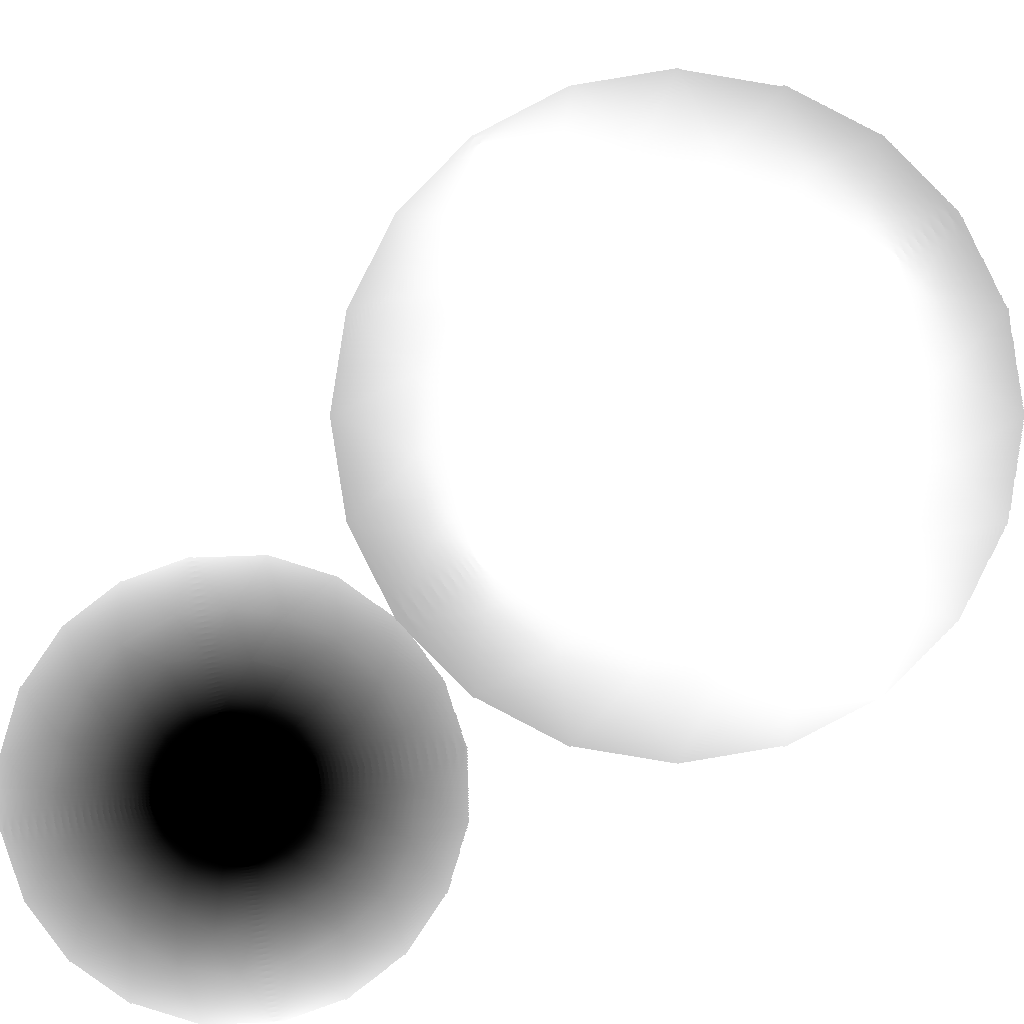
\includegraphics[scale=0.10]{images/final/test/texture_sphere.png} \label{img:final_tex_test_1}}\qquad 
\subfigure[texture piano di prova.obj]{
\includegraphics[scale=0.10]{images/final/test/texture_plan.png} \label{img:final_tex_test_2}} \qquad
\subfigure[texture di teapot.obj]{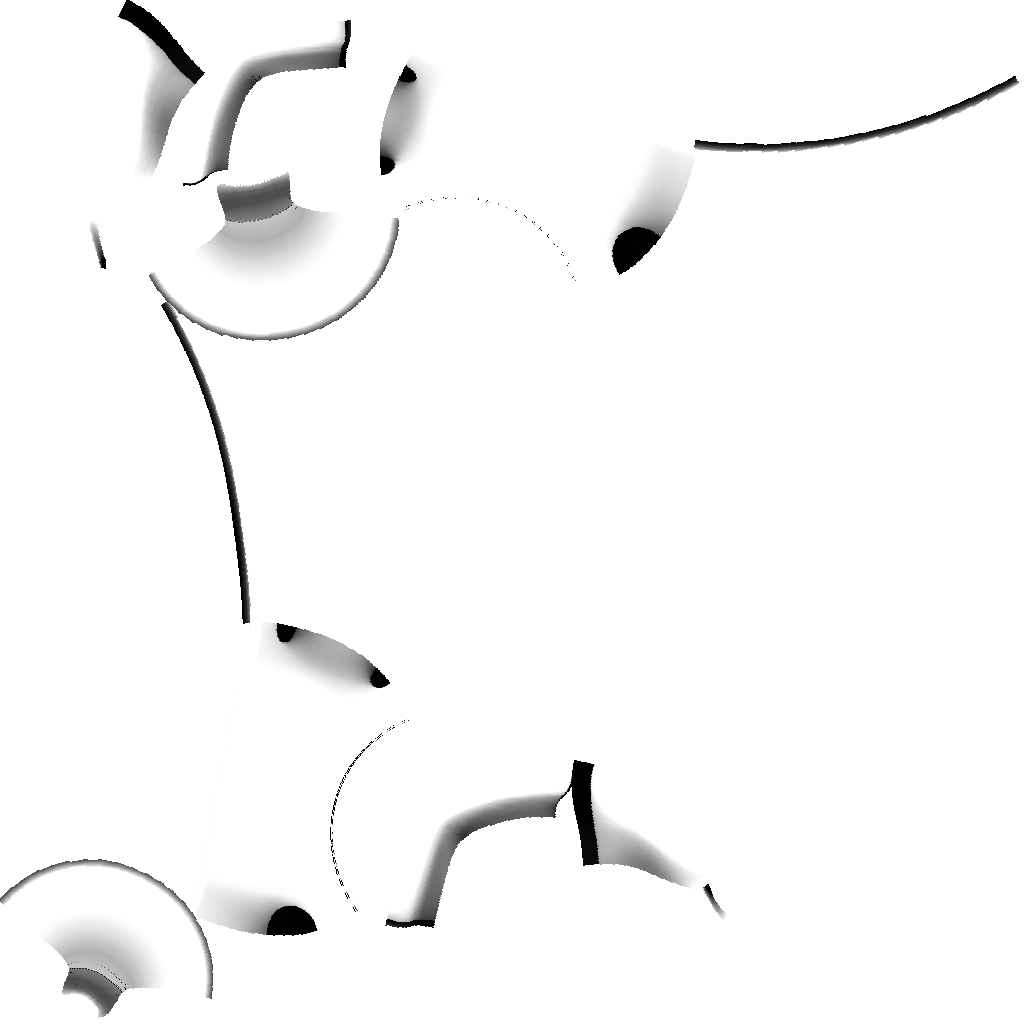
\includegraphics[scale=0.10]{images/final/teapot/texture.png} \label{img:final_tex_teapot}}
\caption{AO texture del modello prova.obj e teapot.obj}
\end{figure}


Il risultato dell'disposizione ottenuta per il modello prova.obj sembra minimizzare lo spazio non utilizzato nel quadrato, possiamo quindi supporre che per questo modello il programma generi una soluzione molto vicina all'ottimo. Mentre la disposizione ottenuta per il modello teapot.obj potrebbe essere sicuramente migliorata.

La \figurename{ \ref{img:final_tex_test_1}, \ref{img:final_tex_test_2}}  e la \figurename{ \ref{img:final_tex_teapot}} rappresentano gli output della fase di calcolo dell'AO texture per i due modelli. Il risultato ovviamente rispecchia sempre ci� che si � ottenuto nella fase di packing. Pi� avanti tratteremo in dettaglio i tempi necessari al calcolo della texture, decisamente influenti in termini di prestazioni.

Il risultato finale per i due modelli si pu� vedere nella \figurename{ \ref{img:final_out}}. In entrambi i casi i problemi riscontrati con la prima versione del programma non si sono presentati se non in minima parte, possiamo quindi concludere che le speculazioni sulle motivazioni alla base delle problematiche riscontrate erano corrette.

\begin{figure}[!h]
\centering %
\subfigure[modello prova.obj]{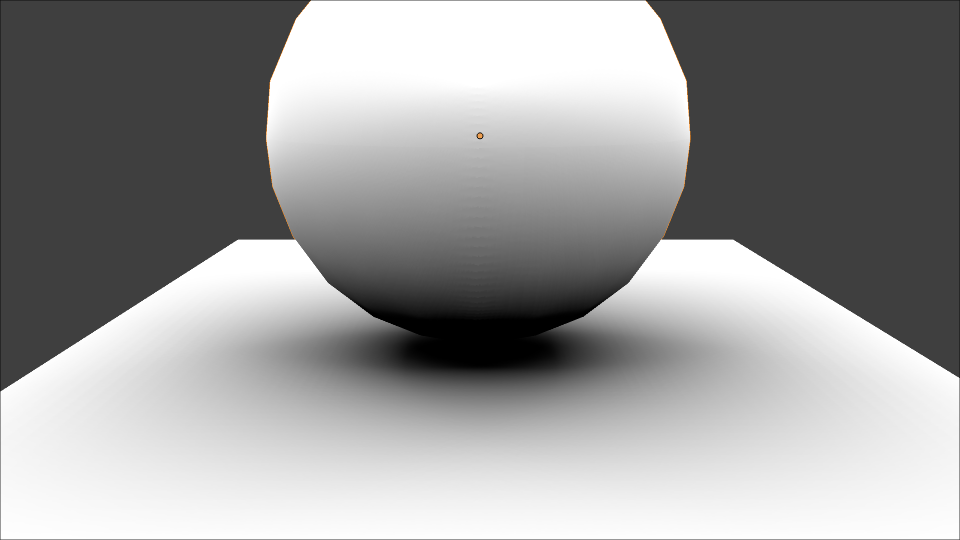
\includegraphics[scale=0.20]{images/final/test/test.png}}\qquad
\subfigure[modello teapot.obj]{\includegraphics[scale=0.20]{images/final/teapot/teapot.png}}
\label{img:final_out}
\caption{output finale}
\end{figure}

\subsection{Test con il modello monkey.obj}
Il test con il modello monkey.obj non ha ottenuto risultati soddisfacenti. La fase in unwrapping non ha ottenuto una parametrizzazione valida per la mesh. Infatti, una sotto-superficie della mesh ha prodotto una mappatura non localmente biunivoca e quindi non valida. Nell'immagine 

\subsection{Tempi di esecuzione}
Le tempistiche di esecuzione sono certamente un punto importante per valutare se il programma � realmente in grado di risolvere il problema. L'obiettivo era quello di valutare il programma nel suo complesso , in particolare nella fase di calcolo della texture e in quella di unwrapping. 

Per valutare le prestazione dell'algoritmo per il calcolo dell'AO texture abbiamo effettuato una serie di test su un unico modello prova.obj. Le prove sono state eseguite impostando diverse risoluzioni per la texture in output, nella \tablename{ \ref{tbl:final_time_tex}} � presente il riepilogo dei dati.

\begin{table}
\centering
\renewcommand\arraystretch{1.3} % aumenta spaziatura tra le righe
\begin{tabular}{p{0.13\textwidth} | p{0.18\textwidth} | p{0.18\textwidth} | p{0.18\textwidth} | p{0.18\textwidth}}
	\textbf{Fase} & \textbf{lato 256px} & \textbf{lato 512px} & \textbf{lato 1024px} & \textbf{lato 2048px} \\
	\hline
	Unwrapping  & 6.5990 s & 6.5830 s & 6.5670 s & 6.5540 s \\

	Packing & 0.8740 s & 0.8730 s & 0.8740 s & 0.8490 s \\

	Texel builder & 3.4470 s & 11.810 s & 42.338 s & 160.73 s \\

	Texture builder & 148.13 s & 473.02 s &  1633.8 s & 6459.5 s \\

	Pulizia memoria & 2.1220 s & 8.7360 s &  33.840 s & 131.50 s \\
	\hline
	Unwrapping  & 1.2790 s & 1.2940 s & 1.2950 s & 1.2950 s \\

	Packing & 0.0160 s & 0.0160 s & 0.0310 s & 0.0150 s \\

	Texel builder & 2.5270 s & 7.7380 s & 27.707 s & 107.23 s \\

	Texture builder & 129.77 s & 502.11 s &  1855.9 s & 7327.7 s \\
	
	Pulizia memoria & 1.8100 s & 9.0010 s &  37.753 s & 152.34 s \\
	\hline
	\textbf{Totale} & 297.05 s (5m) & 1021.7 s (17m) &  3640.9 s (1h) & 14349 s (4h) \\
\end{tabular}
\caption{tempi di esecuzione per il modello prova.obj}
\label{tbl:final_time_tex}
\end{table}

Dai dati ottenuti dal test possiamo osservare che i tempi di esecuzione sono strettamente legati alla dimensione della texture. Possiamo ipotizzare che l'ordine di complessit� dell'algoritmo in funzione della dimensione della texture $d$ sia pari a $O(d^2)$ (considerando trascurabile il tempo necessario per il calcolo della parametrizzazione).

Abbiamo anche effettuato dei test su diverse versioni del modello teapot.obj, ciascun con un numero diverso di triangoli. L'obiettivo era quello di valutare la complessit� legala all'algoritmo di unwrapping, nella \tablename{ \ref{tbl:final_time_unwrapper}} � presente il riepilogo dei dati.
 
\begin{table}
\centering
\renewcommand\arraystretch{1.3} % aumenta spaziatura tra le righe
\begin{tabular}{p{0.13\textwidth} | p{0.18\textwidth} | p{0.18\textwidth} | p{0.18\textwidth} | p{0.18\textwidth}}
	\textbf{Fase} & \textbf{3000 facce} & \textbf{5023 facce} & \textbf{6399 facce} & \textbf{7034 facce} \\
	\hline
	Unwrapping  & 365.00 s & 1237.0 s & 1187.56 s & 1312.0 s \\
\end{tabular}
\caption{tempi di esecuzione per il modello prova.obj}
\label{tbl:final_time_unwrapper}
\end{table}

Dai dati ottenuti dal test non possiamo concludere molto. Sarebbe necessario effettuare pi� prove e su geometrie differenti per ottenere migliori risultati statistici, questo test � quindi da considerare indicativo.

\section{Conclusioni}

Dai test effettuati possiamo trarre alcune considerazioni. Le prove sui modelli prova.obj e teapot.obj hanno portato a dei risultati soddisfacenti dal punto di vista della resa grafica. Mentre la prova sul modello monkey.obj ha evidenziato alcuni problemi nella fase di unwrapping. Le analisi delle tempistiche ha sottolineato la necessit� di migliorare la procedura per il calcolo della texture, pi� avanti suggeriremo come affrontare i problemi che adesso evidenzieremo.

Le problematiche riscontrate nella fase di unwrapping sono principalemente legate alla necessit� di generalizzare ulteriormente il modello di calcolo della parametrizzazione. Il modello monkey.obj ha permesso di evidenziare una situazione che porta alla generazione di una mappatura non localmente biunivoca. L'algoritmo non riesce a determinare una parametrizzazione valida di una superficie della mesh che presenta delle aperture. Abbiamo ipotizzato che probabilmente � questo a portare alla generazione di una soluzione non valida.  

La fase di calcolo della texture non presenta particolari problematiche se non legate ai tempi di esecuzione. Per texture di risoluzione 2048px x 2048px il programma ha bisogno di 4 ore per il calcolo dell'AO texture. Questo pu� diventare problematico se pensiamo che il programma debba calcolare decine di texture. Pensiamo quindi che sia necessario porre l'attenzione anche su questo punto.

La fase di packing influisce notevolmente sulla resa grafica della texture per due ragioni. Il primo motivo � che la disposizione sul piano $O_{uv}$ � direttamente legata alla percentuale di pixel utilizzati per ricoprire il modello. All'aumentare dell'area inutilizzata diminuiscono il numero di pixel utilizzati che vengono applicati sulla superficie e di conseguenza la resa grafica della texture. Il secondo motivo � che la creazione del bordo attorno alle superfici influisce direttamente sulla resa grafica lungo i tagli della mesh. Nell'immagine \ref{img:final_out} si pu� infatti notare la presenza di alcuni tagli neri sulla superficie del modello teapot.obj.

\section{Sviluppi futuri}

In base alle conclusioni appena tratte possiamo suggerire alcuni sviluppi futuri. I suggerimenti riguardano principalmente gli approcci da seguire per risolvere le problematiche appena evidenziate e le migliorie effettuabili sugli algoritmi utilizzati.

Discutiamo ora i possibili approcci da seguire per risolve i problemi riscontrati. Per il problema legato all'unwrapping del modello monkey.obj possiamo pensare di implementare una tecnica per il riconoscimento di superfici forate che provveda alla creazione di riempimenti per questi fori. In questo modo dovrebbe essere possibile parametrizzare la superficie e successivamente scartare i triangoli di riempimento.

Un altro problema riscontrato spesso durante la fase di debug � l'instabilit� dell'algoritmo di packing. In particolare la procedura di creazione del poligono di non sovvrapposizione non � sempre in grado di determinare il vettore di traslazione. Per queste ragioni consigliamo di rivedere l'approccio seguito e magari utilizzare librerie esterne per il calcolo geometrico, sicuramente pi� stabili.

Possiamo pensare di migliorare la fase di calcolo del packing. La procedura implementata effettua il calcolo della disposizione su poligoni convessi, questo non permette di sfruttare a pieno lo spazio a disposizione Un primo miglioramento potrebbe essere ottenuto dalla modifica dell'algoritmo in modo che possa lavorare anche con poligoni convessi. In un secondo momento si potrebbe pensare di aggiungere la possibilit� di effettuare un numero discreto di rotazioni da associare delle figure coinvolte nel packing. In ogni caso consigliamo di migliorare prima la stabilit� numerica dell'algoritmo.

L'algoritmo per il calcolo dell'AO texture trarrebbe dei benifici dal calcolo parallelo. Si potrebbe pensare di realizzare pi� thread in parallelo che lavorano ciascuno su una porzione differente dell'immagine.

%\section{Conclusioni personali}

%\appendix

%\chapter{Prima appendice}


\clearpage

\begin{thebibliography}{9}
\bibitem{cit:nofit} Burke E. K. , Hellier R. S. R. , Kendall G. , Whitwell G. 2007. \emph{Complete and robust No-Fit polygon generation for the irregular stock cutting problem}. European Journal of Operational Research 179, pp. 27-49.
\bibitem{cit:abf} Sheffer A. e De Sturler E. 2001. \emph{Parameterization of faceted surfaces for meshing using angle based flatteling}. Engin. Comput. 17, 326-337.
\bibitem{cit:ipopt} W�chter A. and Biegler L. T. 2006. \emph{On the Implementation of a Primal-Dual Interior Point Filter Line Search Algorithm for Large-Scale Nonlinear Programming}. Mathematical Programming 106(1), pp. 25-57. 
\end{thebibliography}

    	

\end{document}
